\chapter{The CHIPS R\&D project} %%%%%%%%%%%%%%%%%%%%%%%%%%%%%%%%%%%%%%%%%%%%%%%%%%%%%%%%%%%%%%%%%
\label{chap:chips} %%%%%%%%%%%%%%%%%%%%%%%%%%%%%%%%%%%%%%%%%%%%%%%%%%%%%%%%%%%%%%%%%%%%%%%%%%%%%%%

In pursuit of answers to the open questions presented in the previous chapter, neutrino
experiments are clearly becoming increasingly, and possibly prohibitively, expensive and
impractical. This trend is particularly true of the next generation of long-baseline experiments,
DUNE and Hyper-Kamiokande, with cost estimates reaching billions of dollars and construction times
of greater than half a decade. It is also telling that the vast majority of global research effort
goes into just these two future projects, such is their complexity, cost, and lead time.

It is evident that for detectors to remain practical and affordable into the future, a novel
design strategy is highly desirable. This approach is especially the case if megaton scale
detectors are ever to become a reality. While instrumentation will continue to steadily improve
with time, the statistics of low event counts will always limit neutrino experiments until vastly
larger detectors can be built. Therefore, R\&D efforts must focus on such detectors now, whilst
also attempting to complement the current and upcoming generation of experiments.

The \chips R\&D project~\cite{adamson2013} aims to develop novel strategies and technologies for
very large yet practical `cheap as chips' water Cherenkov detectors. Primarily aimed for
deployment in long baseline accelerator beam scenarios, \chips aims to lower the cost per kt of
sensitive mass to between \$200k-\$300k. For comparison, the Super-Kamiokande detector cost
approximately \$4 million per kt to build. As physics sensitivity depends on more than just
sensitive mass, this comparison is not entirely rigorous; however, it highlights the scale of
possible cost savings.

This chapter aims to describe the fundamental aspects of the \chips R\&D project in detail.
Firstly, the \chips concept will be outlined along with both neutrino beam and Cherenkov detector
physics for context. The design, construction, deployment, and status of the \chipsfive prototype
detector will then follow. Finally, a description of the Monte Carlo methods used to simulate
\chips detectors such as \chipsfive is given, alongside how input neutrino events are generated.

\section{The CHIPS concept} %%%%%%%%%%%%%%%%%%%%%%%%%%%%%%%%%%%%%%%%%%%%%%%%%%%%%%%%%%%%%%%%%%%%%%
\label{sec:chips_concept} %%%%%%%%%%%%%%%%%%%%%%%%%%%%%%%%%%%%%%%%%%%%%%%%%%%%%%%%%%%%%%%%%%%%%%%%

The \chips concept is to deploy cylindrical water Cherenkov detector modules into deep bodies of
water on the Earth's surface such as lakes, reservoirs, and flooded mine pits. Initially
constructed on land, \chips detectors can be floated into position before being sunk. The water
above the sunken detector provides a modest overburden from cosmic rays, whilst the surrounding
water provides support for a lightweight detector structure. By removing the need for underground
excavation and expensive structural support, the cost of construction can be dramatically reduced.

Additionally, the common practice of building majority bespoke components is replaced by using
modern commercially available components wherever possible. The number of expensive elements, such
as photomultiplier tubes are also reduced by only considering multi-$\GeV$ accelerator beam
neutrino events, such that full high density detector instrumentation is not required.

Furthermore, \chips detectors are not only designed to be cheap, but practical. Easy to build,
quick to deploy, and upgradable once operational, multiple detector modules can be flexibly
combined depending on available resources and funding. When compared to DUNE and Hyper-Kamiokande
both which require a large upfront budget and many years to construct, cheap \chips detector
modules can be deployed as needed in under a year by a relatively small team.

To date, \chips R\&D efforts have been based in the USA to exploit the \numi beam before the end
of its lifetime. Plans are focused on the scaling of \chips detectors for the deployment of
multiple modules within the LBNF beam once operational. Collaborators from primarily University
College London, The University of Wisconsin Madison, and Nikhef are focused on multiple R\&D
efforts, each aiming to prove the viability of a crucial component of the \chips concept.

\begin{itemize}
    \item \textbf{Detector construction:} Aiming to prove that the construction and deployment of
          \chips concept detector modules is possible. Two prototype detectors have so far been
          deployed. Firstly, the small \chipsm module shown in Fig.~\ref{fig:chips_m}, deployed
          into a flooded mine pit in northern Minnesota during the summer of 2014~\cite{perch2015,
          pfutznerProto2017, pfutzner2017}. Secondly, the much larger \unit{5}{\text{kt}}
          \chipsfive module, deployed into the same pit during the summer of 2019 and detailed in
          Section.~\ref{sec:chips_detector}.

    \item \textbf{Water filtration:} Aiming to prove that adequate water purity can be achieved
          using cheap, commercially available filtration. Extensive studies have proven that by
          filtering water directly from bodies of water on the Earth's surface (including flooded
          mine pits), adequate photon attenuation lengths greater than \unit{100}{\text{m}} are
          achievable~\cite{amat2017, campbell2020}.

    \item \textbf{Physics sensitivity:} Aiming to prove that \chips concept detector modules (even
          the prototypes) can provide significant physics contributions alone or alongside the
          current and next generation of experiments. Single modules in the current \numi beam
          (discussed in Section.~\ref{sec:chips_concept_beam}) and multiple modules in the future
          LBNF beam have been studied~\cite{pfutzner2017, adde2016, lang2015}.

    \item \textbf{Data acquisition:} Aiming to prove that a cheap data acquisition (DAQ) system
          using commercially available components and software is viable~\cite{eijk2018}. Outlined
          in Chapter.~\ref{chap:daq}, \chips implements a novel use of cheap single-board
          computers to collect photomultiplier tube data.

    \item \textbf{Event reconstruction and classification:} Aiming to prove that modern machine
          learning techniques can be successfully applied to large water Cherenkov concepts such
          as \chips. The primary contribution of this thesis (detailed in Chapter.~\ref{chap:cnn}
          and Chapter.~\ref{chap:results}), this work feeds directly into both the physics
          sensitivity studies mentioned above and detector design optimisation.
\end{itemize}

\begin{figure} % CHIPS-M DIAGRAM %
    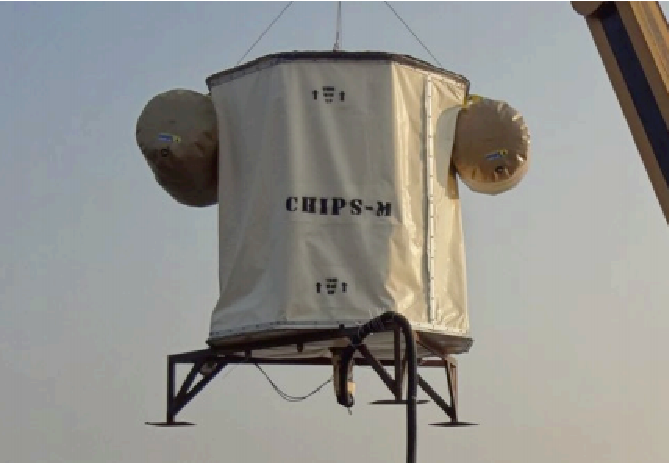
\includegraphics[width=0.6\textwidth]{diagrams/4-chips/chips_m.pdf}
    \caption[Picture of the \chipsm detector just before deployment]
    {Picture of the \unit{3.3}{\text{m}} high \chipsm detector just before deployment. Temporary
        floatation bags are attached to the top rim of the detector, while the umbilical cord
        carrying data, power, and filtered water is attached to the base.}
    \label{fig:chips_m}
\end{figure}

\subsection{The neutrino beam} %%%%%%%%%%%%%%%%%%%%%%%%%%%%%%%%%%%%%%%%%%%%%%%%%%%%%%%%%%%%%%%%%%%
\label{sec:chips_concept_beam} %%%%%%%%%%%%%%%%%%%%%%%%%%%%%%%%%%%%%%%%%%%%%%%%%%%%%%%%%%%%%%%%%%%

\chips detectors will primarily study the appearance of $\nu_{e}$ oscillating from $\nu_{\mu}$
over a long-baseline. To generate a sufficient number of GeV scale $\nu_{\mu}$, a high-intensity
accelerator beam is required. Currently, only two such beams exist, the J-PARC based beam in Japan
used by the T2K experiment and the \numi beam in the USA used by \nova. Here we describe the \numi
beam~\cite{adamson2016} as it is directly relevant to current \chips efforts. However, it is
essential to note that \chips detectors are designed to be deployed into any high-intensity
neutrino beam, including the future \numi replacement, LBNF.

The \numi beam is an accelerator muon neutrino beam produced at Fermilab near Chicago in the USA.
Beginning operation in 2005 for the MINOS experiment, \numi was upgraded in 2013 to provide a
higher intensity and energy, principally to achieve a peak in neutrino energy near the
$\sim$\unit{1.5}{\GeV} $\nu_{\mu}\rightarrow\nu_{e}$ oscillation maximum for \nova. Currently, the
\numi beam achieves an intensity of \unit{700}{\text{kW}} (\unit{740}{\text{kW}} at peak) making
it the most powerful such beam in the world. A schematic of the \numi beamline configuration is
shown in Fig.~\ref{fig:numi_beam}.

\begin{figure} % NUMI BEAM DIAGRAM %
    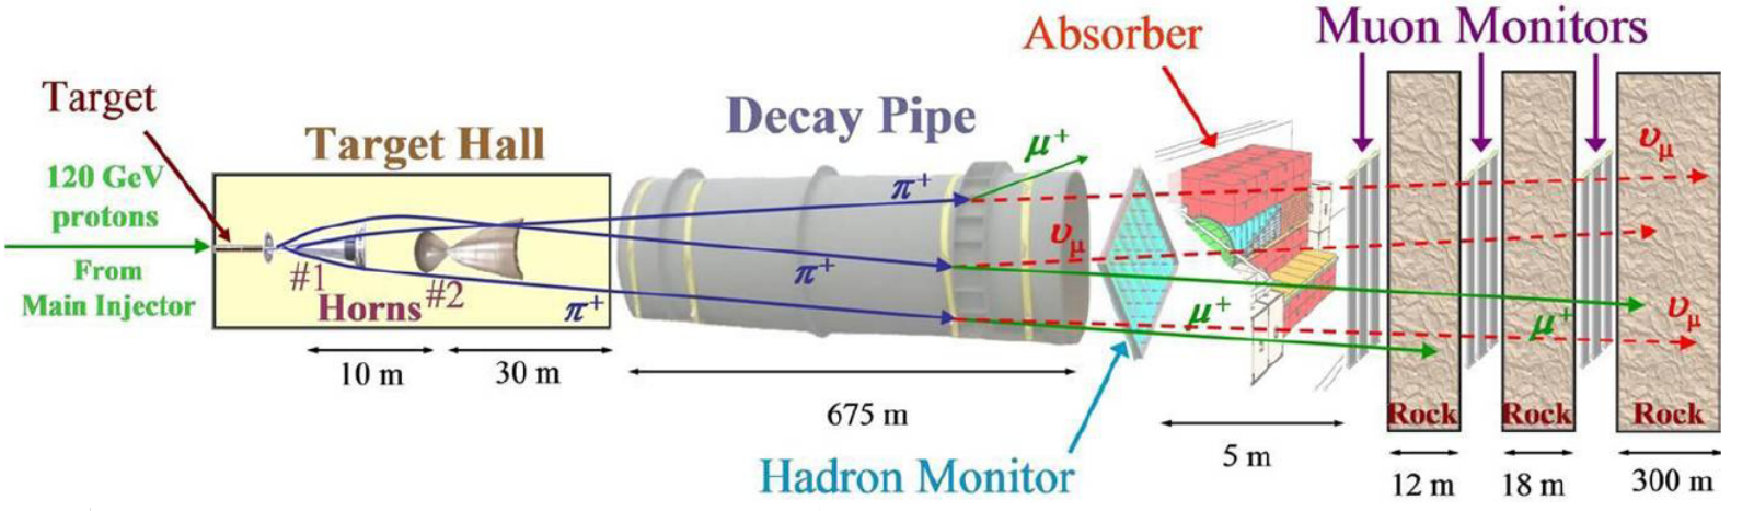
\includegraphics[width=\textwidth]{diagrams/4-chips/numi_beam.pdf}
    \caption[Schematic of the main components of the \numi beamline]
    {Schematic of the main components of the \numi beamline. The MINOS and \nova near detectors
        and the MINERvA experiment are located just to the right of what is shown. Figure taken
        from Ref.~\cite{adamson2016}.}
    \label{fig:numi_beam}
\end{figure}

Every \unit{1.33}{\text{seconds}} a \unit{10}{\micro\text{s}} long spill of protons accelerated to
\unit{120}{\GeV} by the Main Injector ring are directed towards a stationary graphite target. The
resulting interactions create a shower of hadrons containing predominantly pions and kaons. The
hadrons are passed through a focusing system of two magnetic horns tuned principally to focus
positively charged pions along the beamline while rejecting other particles. After focusing, any
surviving hadrons are allowed to decay in flight to a beam of muon neutrinos in a
\unit{675}{\text{m}} long decay pipe via the processes:
\begin{align} % NUMI DECAY EQUATIONS %
    \pi^{+} & \rightarrow\mu^{+}+\nu_{\mu}, \label{eq:pi_decays}   \\
    K^{+}   & \rightarrow\mu^{+}+\nu_{\mu}. \label{eq:kaon_decays}
\end{align}
The resulting muons also decay such that $\mu^{+}\rightarrow e^{+}+\nu_{e}+\bar{\nu}_{\mu}$,
producing an intrinsic $\nu_{e}$ component as well as wrong sign $\nu_{\mu}$ contamination.

Alternatively, the polarity of the horns can be used to switch the dominant sign of the hadrons
focused, allowing \numi to operate as either a neutrino or antineutrino beam. These two modes of
operation are called \emph{forward horn current} and \emph{reverse horn current} for primarily a
neutrino or antineutrino beam composition respectively. Any remaining hadrons, alongside
electrons, muons and surviving primary protons are absorbed by rock downstream of the decay pipe,
leaving just the neutrino components of the beam.

Long-baseline neutrino experiments typically consist of a \emph{near} detector to measure the
neutrino composition at source and a much larger \emph{far} detector to measure the oscillated
composition after many hundreds of kilometres. The \numi beamline contains three detectors after
\unit{300}{\text{m}} of rock: The MINERvA spectrometer~\cite{mcfarland2006}, the near detector for
MINOS (now used by MINERvA), and the near detector for \nova. \chips prototypes within the \numi
beam will not have a dedicated near detector; therefore, data from the above detectors will be
crucial for physics analysis in order to constrain the beam composition and flux.

The \numi neutrino beam passes through the Earth's crust until it finally emerges in northern
Minnesota. This is where the MINOS, \nova, and prototype \chips far detectors are located (used to
be located in the MINOS case), as shown in Fig.~\ref{fig:numi_map}. The Minnesota state nickname
`land of 10,000 lakes' is not an overstatement, with a vast number of potential lakes for \chips
detector deployment. Additionally, intense iron ore mining on the `Iron Range' provides many
suitable disused (and now flooded) mine pits. The exact \chipsfive prototype detector location is
discussed in greater detail within Section.~\ref{sec:chips_detector_location}.

\begin{figure} % CHIPS LOCATION IN NUMI DIAGRAM %
    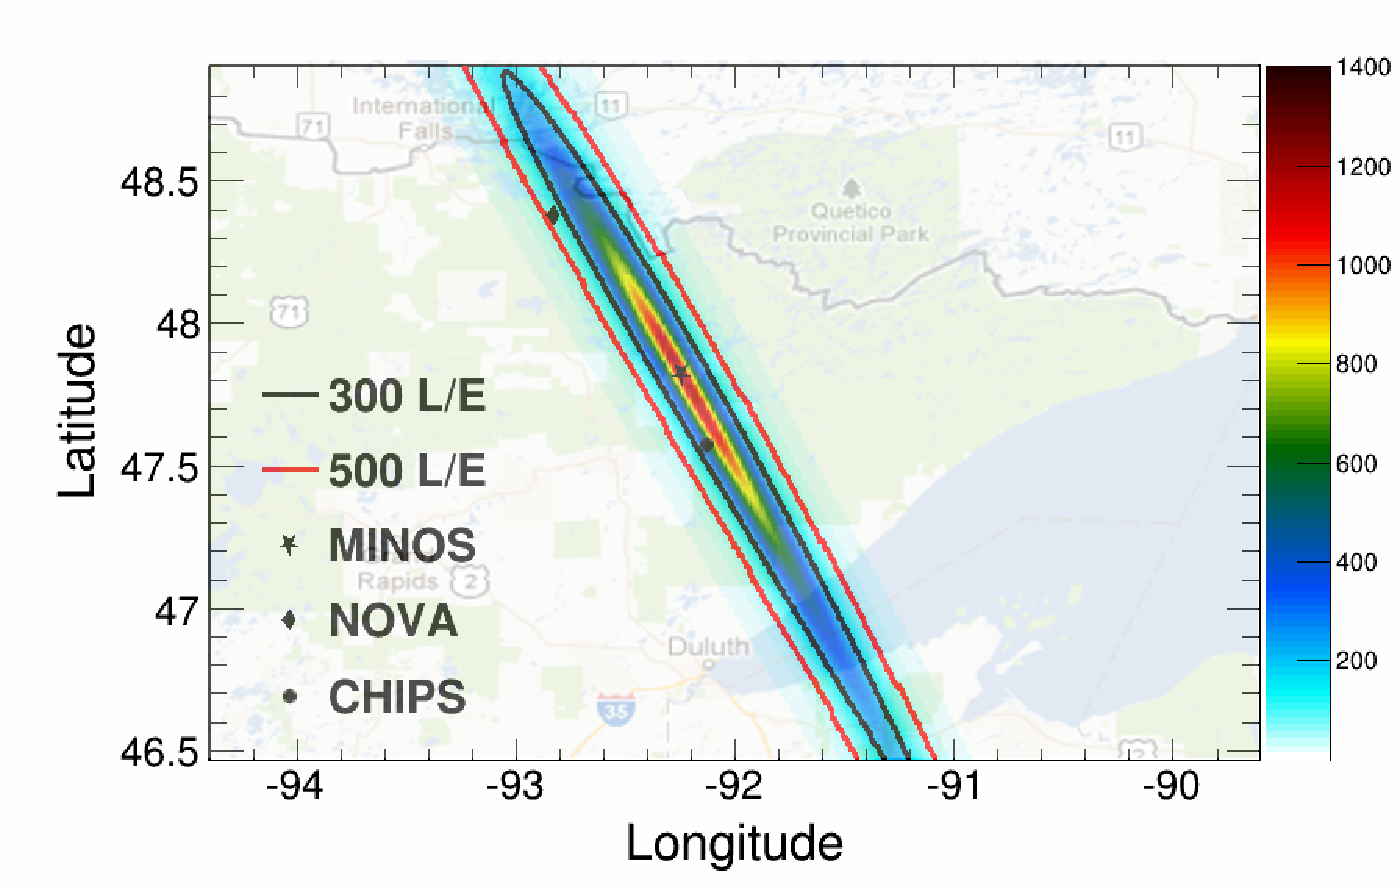
\includegraphics[width=0.7\textwidth]{diagrams/4-chips/numi_map.pdf}
    \caption[Map of detector locations in the \numi beam]
    {Map of the MINOS, \nova and \chips locations in the \numi beam as it surfaces in northern
        Minnesota. Shown is the expected neutrino event rate assuming no oscillations, with lines
        of constant L/E indicated with contours. The western extent of Lake Superior can be seen
        in the lower right of the map for reference. Image taken from Ref.~\cite{adamson2013}.}
    \label{fig:numi_map}
\end{figure}

Due to the kinematics of pion decay, whether the far detector is placed directly on the beam axis
or not can have a significant impact on the observed energy spectrum of beam neutrinos, as shown
in Fig.~\ref{fig:numi_axis}. For neutrinos directly on the beam axis, there is a strong dependence
on the energy of the parent pion within Eq.~\ref{eq:pi_decays}. However, as the off-axis angle
increases, the neutrino energy becomes less and less dependent on the parent pion energy and is
restricted to a narrowing range of decreasing energies. 

Known as the \emph{off-axis effect} this phenomenon is used by both \nova and T2K to create a
narrow energy peak focused on the important $\nu_{\mu}\rightarrow\nu_{e}$ oscillation maximum. By
reducing the tail of high energy neutrinos, the number of background NC events can also be greatly
reduced, as is the case for the \unit{7}{\text{mrad}} off-axis \chipsfive detector module.

\begin{figure} % OFF-AXIS FLUX DIAGRAM %
    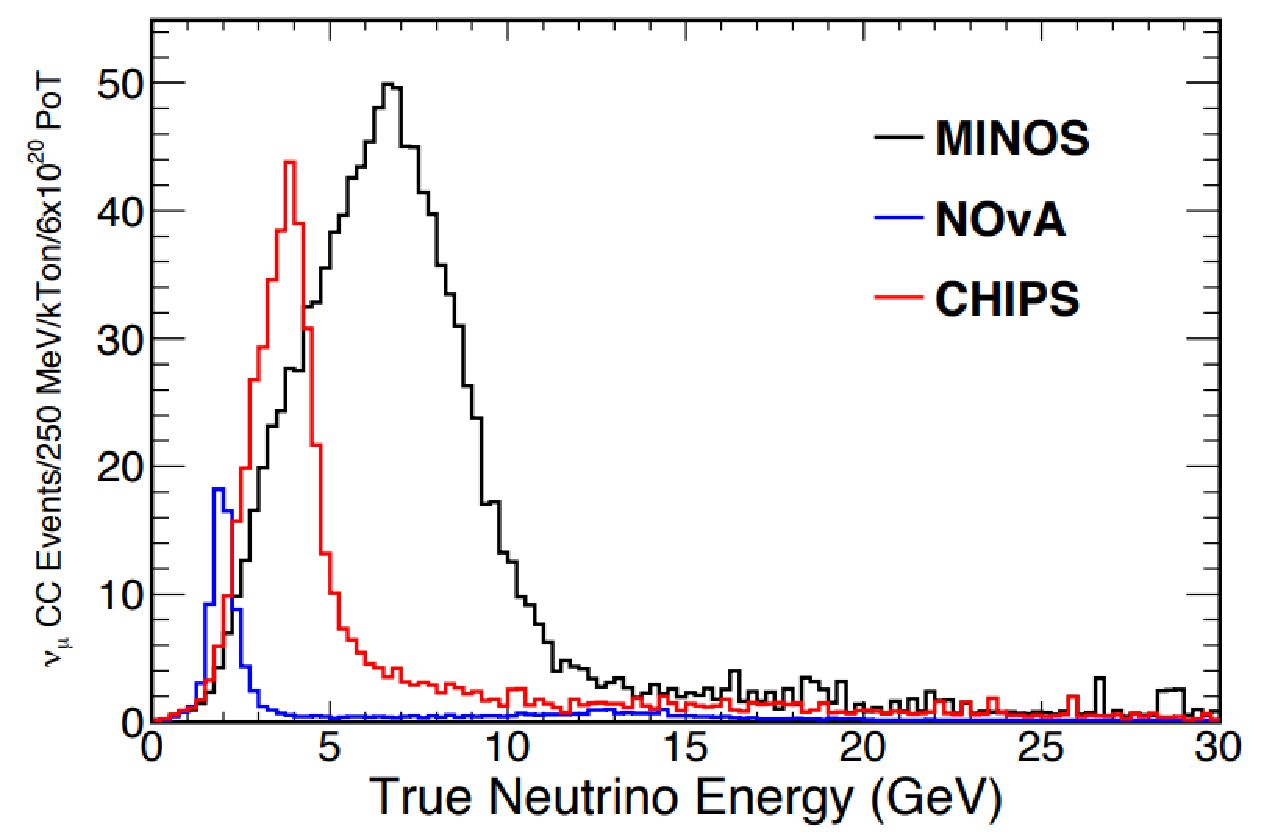
\includegraphics[width=0.6\textwidth]{diagrams/4-chips/numi_axis.pdf}
    \caption[Muon neutrino flux for different \numi detectors at different off-axis angles]
    {Muon neutrino flux for different \numi detectors at different off-axis angles. Shown are the
        neutrino energy spectrums for MINOS (on-axis), \chipsfive (\unit{7}{\text{mrad}}
        off-axis), and \nova (\unit{14}{\text{mrad}} off-axis). Figure taken from
        Ref.~\cite{adamson2013}.}
    \label{fig:numi_axis}
\end{figure}

\subsection{Water Cherenkov detectors} %%%%%%%%%%%%%%%%%%%%%%%%%%%%%%%%%%%%%%%%%%%%%%%%%%%%%%%%%%%
\label{sec:chips_concept_cherenkov} %%%%%%%%%%%%%%%%%%%%%%%%%%%%%%%%%%%%%%%%%%%%%%%%%%%%%%%%%%%%%%

The \chips detector concept is based upon the water Cherenkov technique for neutrino detection. A
large body of target water is instrumented with photomultiplier tubes (PMTs) to record the
Cherenkov radiation produced by sufficiently relativistic charged particles produced in neutrino
interactions. By using readily available water as the target material and only instrumenting the
surface of the volume, water Cherenkov detectors provide the best detection methodology for
maximising volume and reducing cost.

Cherenkov radiation is emitted by all electrically charged particles travelling faster than the
local phase velocity of light in a dielectric medium. Similar to the sonic boom created by a
supersonic aircraft, Cherenkov radiation forms a shock wave of coherent light, as shown in
Fig.~\ref{fig:cherenkov}. Typically, the emitted light has wavelengths in the optical to
ultraviolet range ($\sim400~\text{nm}$). When projected onto the detector wall, the resulting cone
of radiation generates a distinctive ring shape. The cone opening angle (the angle at which light
is emitted) $\theta_{c}$ is given by
\begin{equation}
    \cos\theta_{c} = \frac{1}{\beta n(\lambda)},
    \label{eq:cherenkov_angle}
\end{equation}
where $\beta=v/c$ and $n$ is the refractive index of the medium~\cite{particle2020}. Note that $n$
is a function of the wavelength of emission $\lambda$, and so is the opening angle. As the
refractive index of water is $\sim 1.33$ for typical wavelengths of emission, and using the
ultrarelativistic limit $\beta\sim 1$ the opening angle is found to be $\sim41^{\circ}$.

\begin{figure} % CHERENKOV EFFECT DIAGRAM DIAGRAM %
    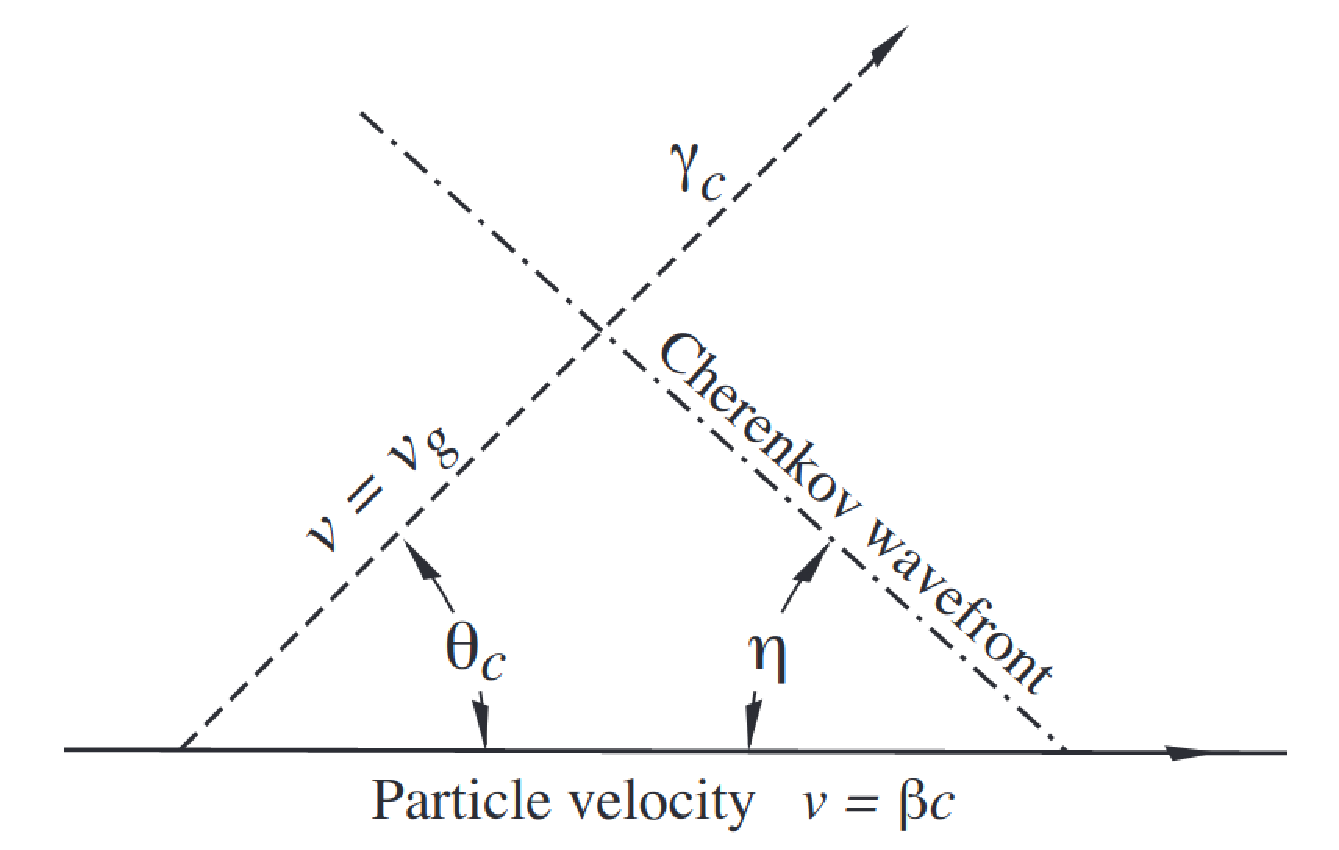
\includegraphics[width=0.6\textwidth]{diagrams/4-chips/cherenkov.pdf}
    \caption[Diagram of Cherenkov radiation emission]
    {Diagram of Cherenkov radiation emission and wavefront angles. The angles $\theta_{c}$ and
        $\eta$ are not equal in a dispersive medium. Figure taken from Ref.~\cite{particle2020}}
    \label{fig:cherenkov}
\end{figure}

In Eq.~\ref{eq:cherenkov_angle} there is no Cherenkov emission when $\cos\theta_{c} > 1$, which is
the case when $\beta n(\lambda)<1$. Therefore, a Cherenkov energy threshold $E_{t}$ exists for
charged particles. When expressed in terms of the particle mass $m$, the threshold is given by
\begin{equation}
    E_{t} = \gamma m = \frac{m}{\sqrt{1-(1/n)^{2}}}.
    \label{eq:cherenkov_threshold}
\end{equation}
Again using $n\sim 1.33$, a threshold energy of $\sim1.5~m$ is typical.

The number of Cherenkov photons emitted by a particle of charge $ze$ per unit wavelength per unit
path length is given by
\begin{equation}
    \frac{d^{2}N}{d\lambda dx}=\frac{2\pi\alpha z^{2}}{\lambda^{2}}
    \left(1-\frac{1}{1-\beta^{2}n^{2}(\lambda)}\right),
    \label{eq:cherenkov_emission}
\end{equation}
where $\alpha$ is the fine structure constant ($\sim1/137$)~\cite{particle2020}. Integrating over
the range of wavelengths for which PMTs are typically sensitive, \unit{350}{\text{nm}} to
\unit{650}{\text{nm}}, and using $\beta\sim 1$ and $n\sim 1.33$ gives approximately $240$ photons
emitted per cm travelled by the charged particle~\cite{perch2017}.

By analysing the Cherenkov rings of light recorded by the PMTs on the walls of the detector,
information about the charged particles within an event can be determined. The underlying neutrino
interaction can then be understood indirectly. Primarily, the challenge for accelerator beam water
Cherenkov detectors is the identification and reconstruction of an electron or muon ring likely to
have been produced from a beam neutrino and not a cosmic ray. This event topology indicates a beam
CC $\nu_{e}$ or CC $\nu_{\mu}$ event respectively, rejecting NC and cosmic events.

The basic shape of a Cherenkov ring can be used to tell which charged particle created it. Muons
are long-lived and typically travel many metres within the detector, producing a clean ring with
sharp edges as is shown in Fig.~\ref{fig:cc_numu_event}. Conversely, electrons almost immediately
initiate an electromagnetic shower; therefore, the observed ring is the sum of multiple rings
produced from the individual electrons and positrons within the shower. As a consequence, when
compared to a muon ring, electron rings are characteristically fuzzy, as is shown in
Fig.~\ref{fig:cc_nue_event}. A factor of this difference can be seen in Fig.~\ref{fig:emission
distance}, which shows how the total amount of Cherenkov radiation is emitted for both electrons
and muons as a function of distance from the interaction vertex.

\begin{figure} % SIMULATED EVENT DISPLAY DIAGRAM %
    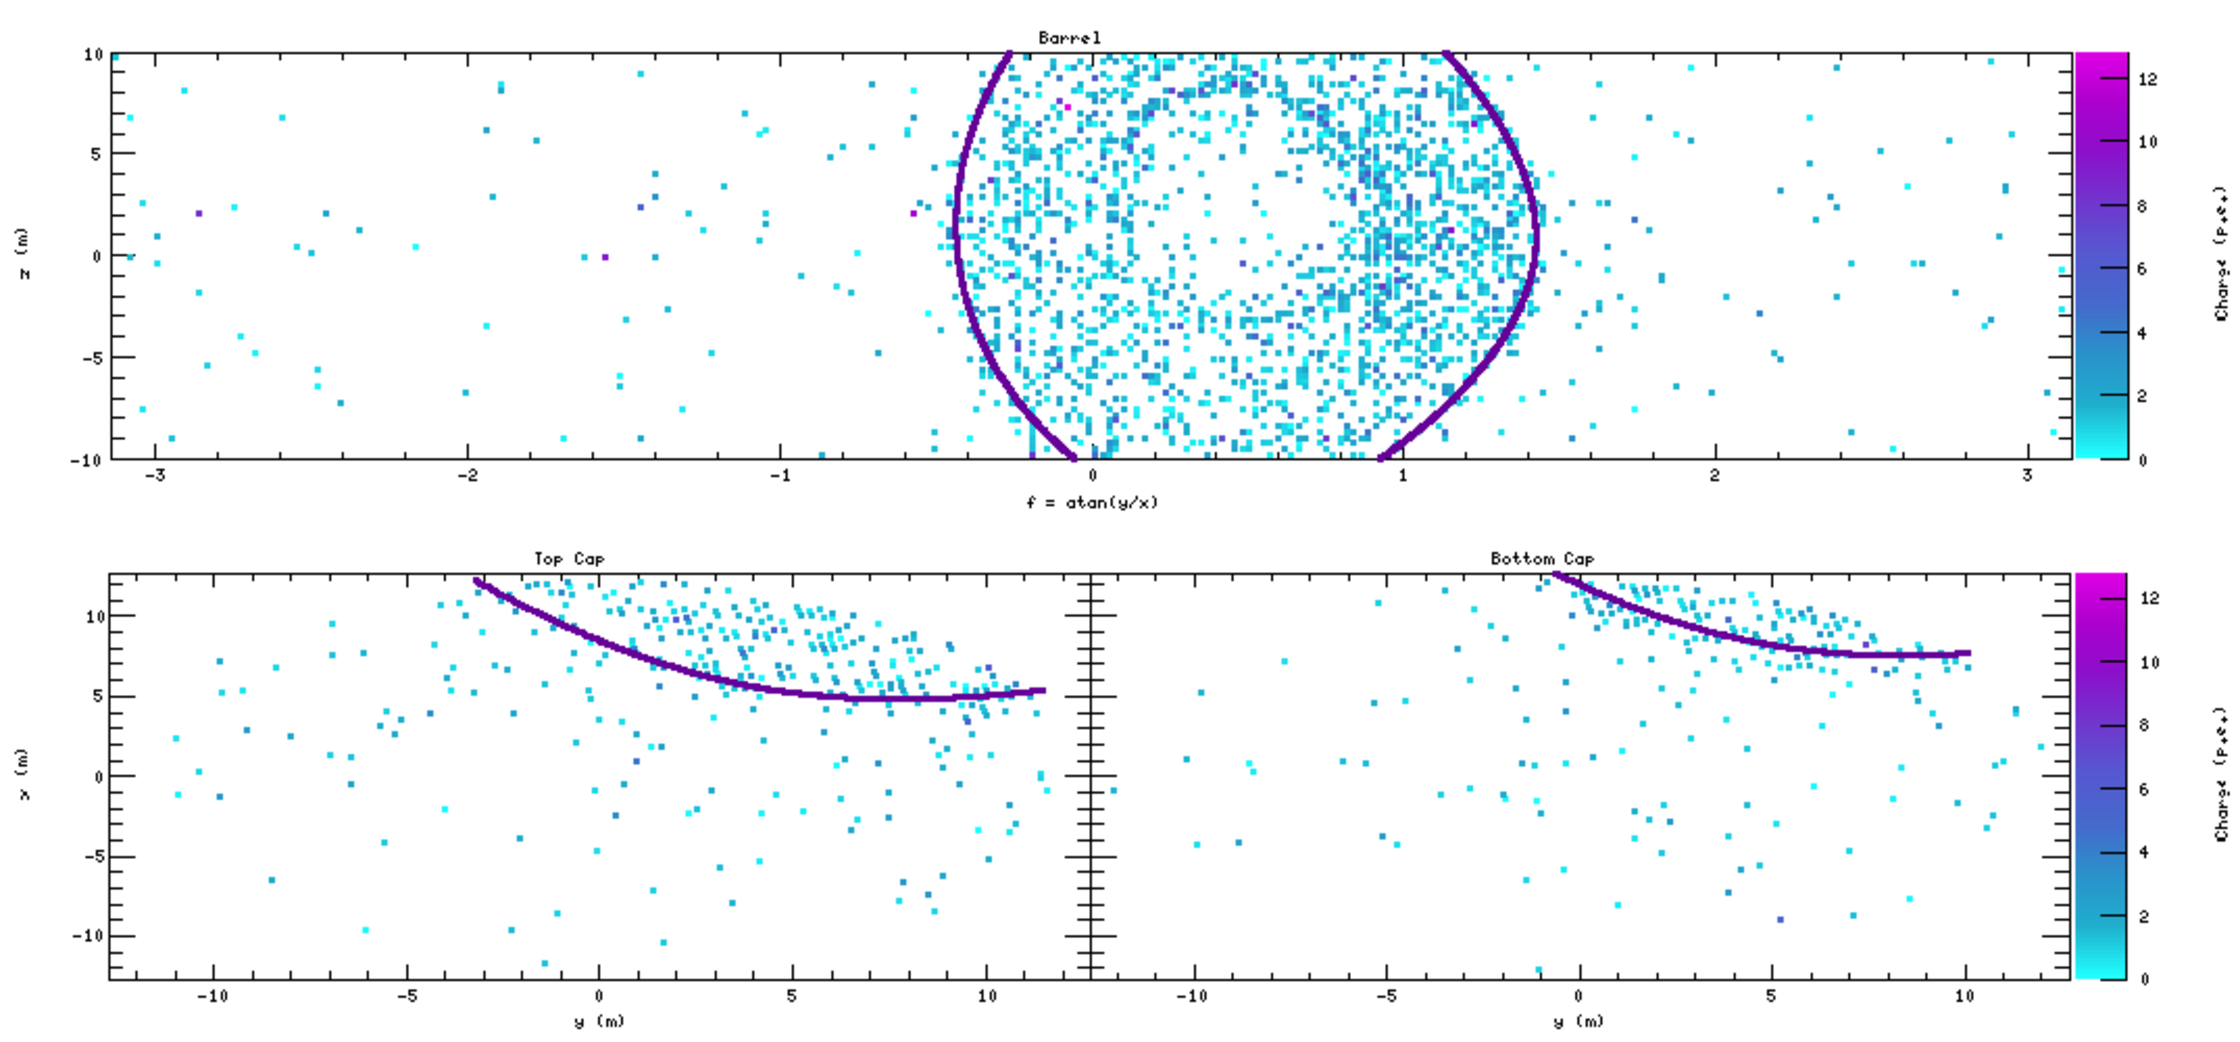
\includegraphics[width=\textwidth]{diagrams/4-chips/cc_numu_event.pdf}
    \caption[Event display of a simulated beam CC $\nu_{\mu}$ event]
    {Event display of a simulated beam CC $\nu_{\mu}$ quasi-elastic event with a single muon in
        the final state of energy \unit{2.36}{\GeV}. Both the unrolled barrel and endcaps are
        shown with every entry representing a hit PMT with the colour indicating the collected
        charge. The purple ring indicates the true muon Cherenkov cone projected onto the detector
        walls.}
    \label{fig:cc_numu_event}
\end{figure}

\begin{figure} % SIMULATED EVENT DISPLAY DIAGRAM %
    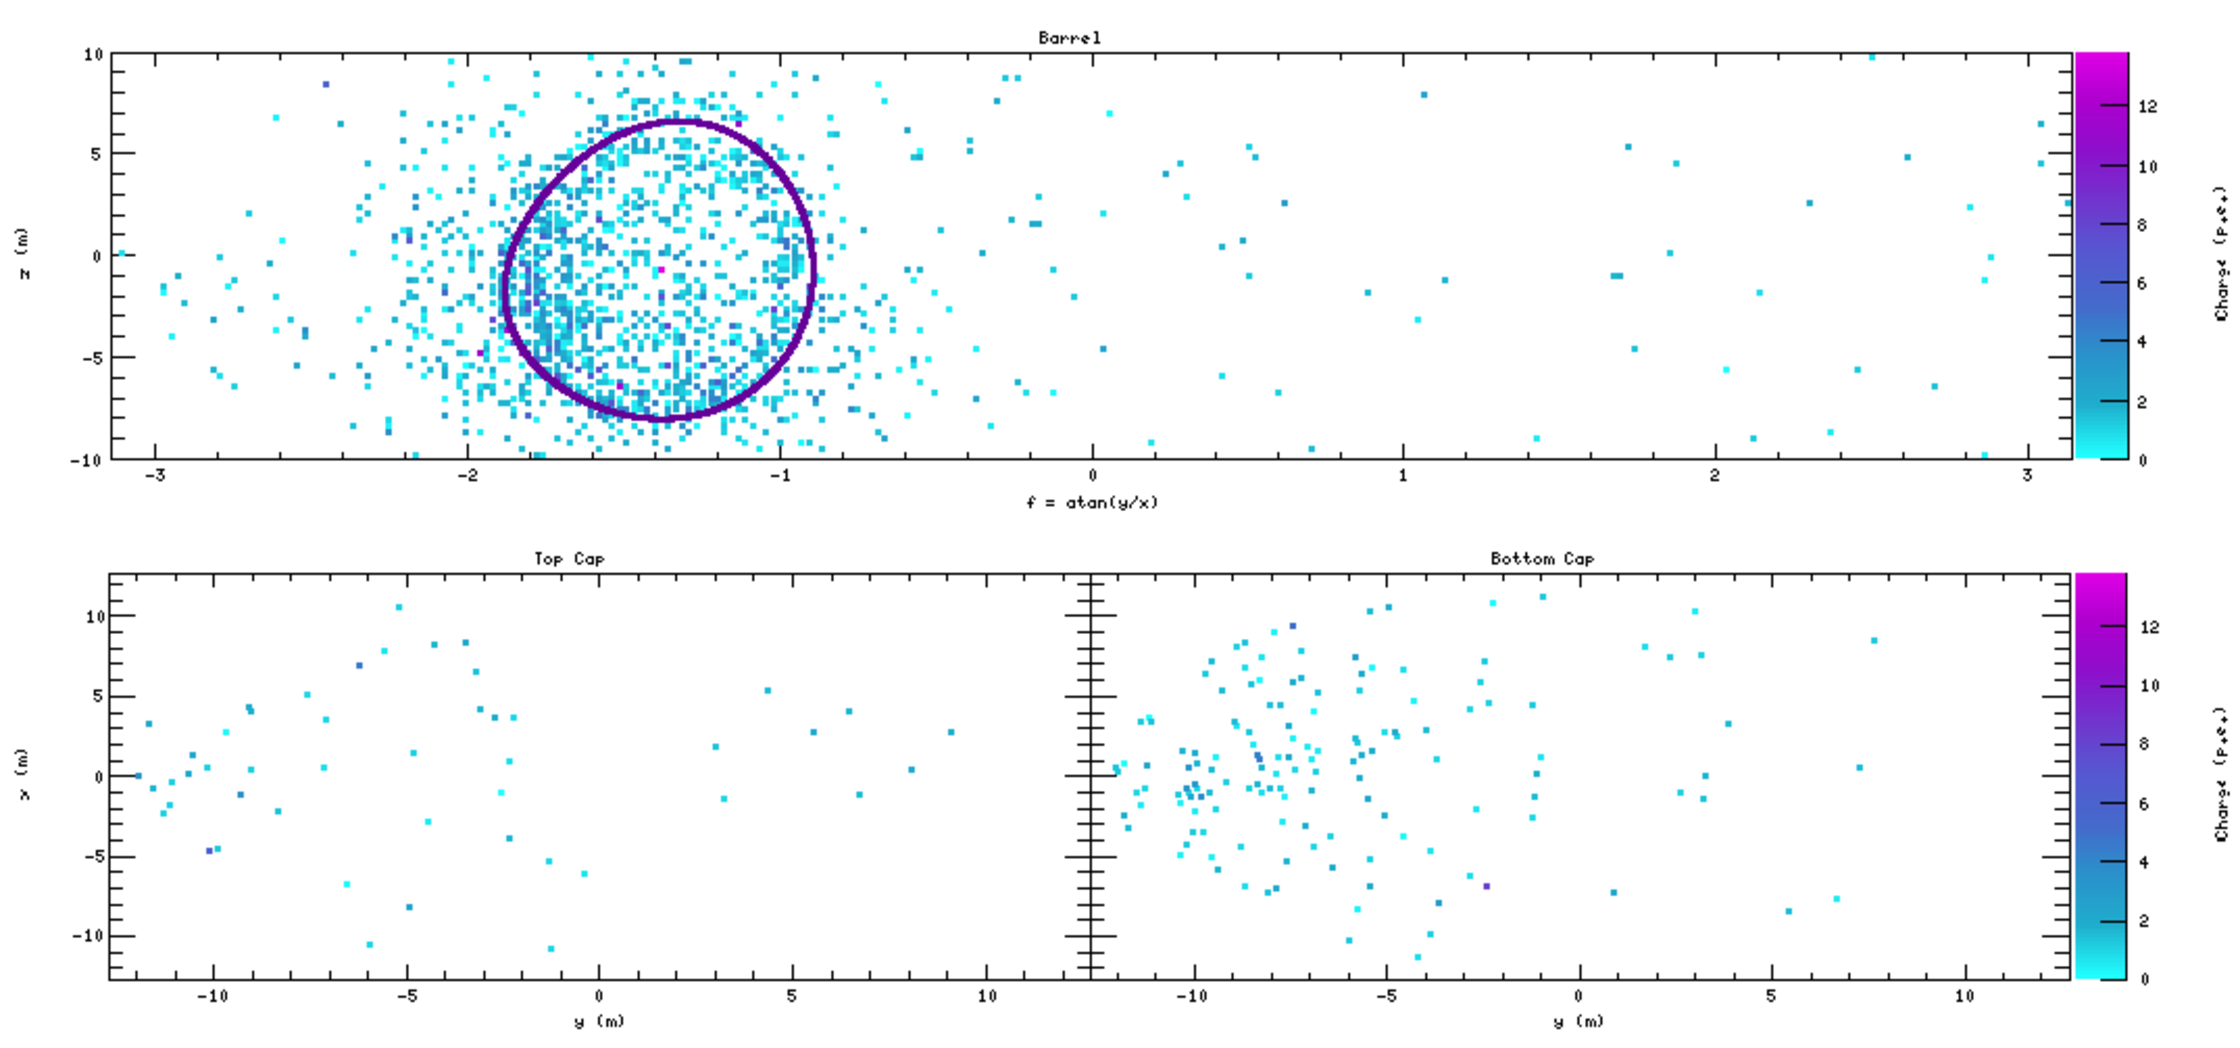
\includegraphics[width=\textwidth]{diagrams/4-chips/cc_nue_event.pdf}
    \caption[Event display of a simulated beam CC $\nu_{e}$ event]
    {Event display of a simulated beam CC $\nu_{e}$ quasi-elastic event with a single electron in
        the final state of energy \unit{1.05}{\GeV}. Both the unrolled barrel and endcaps are
        shown with every entry representing a hit PMT with the colour indicating the collected
        charge. The purple ring indicates the true electron Cherenkov cone projected onto the
        detector walls.}
    \label{fig:cc_nue_event}
\end{figure}

\begin{figure} % EMISSION DISTANCE DIAGRAM %
    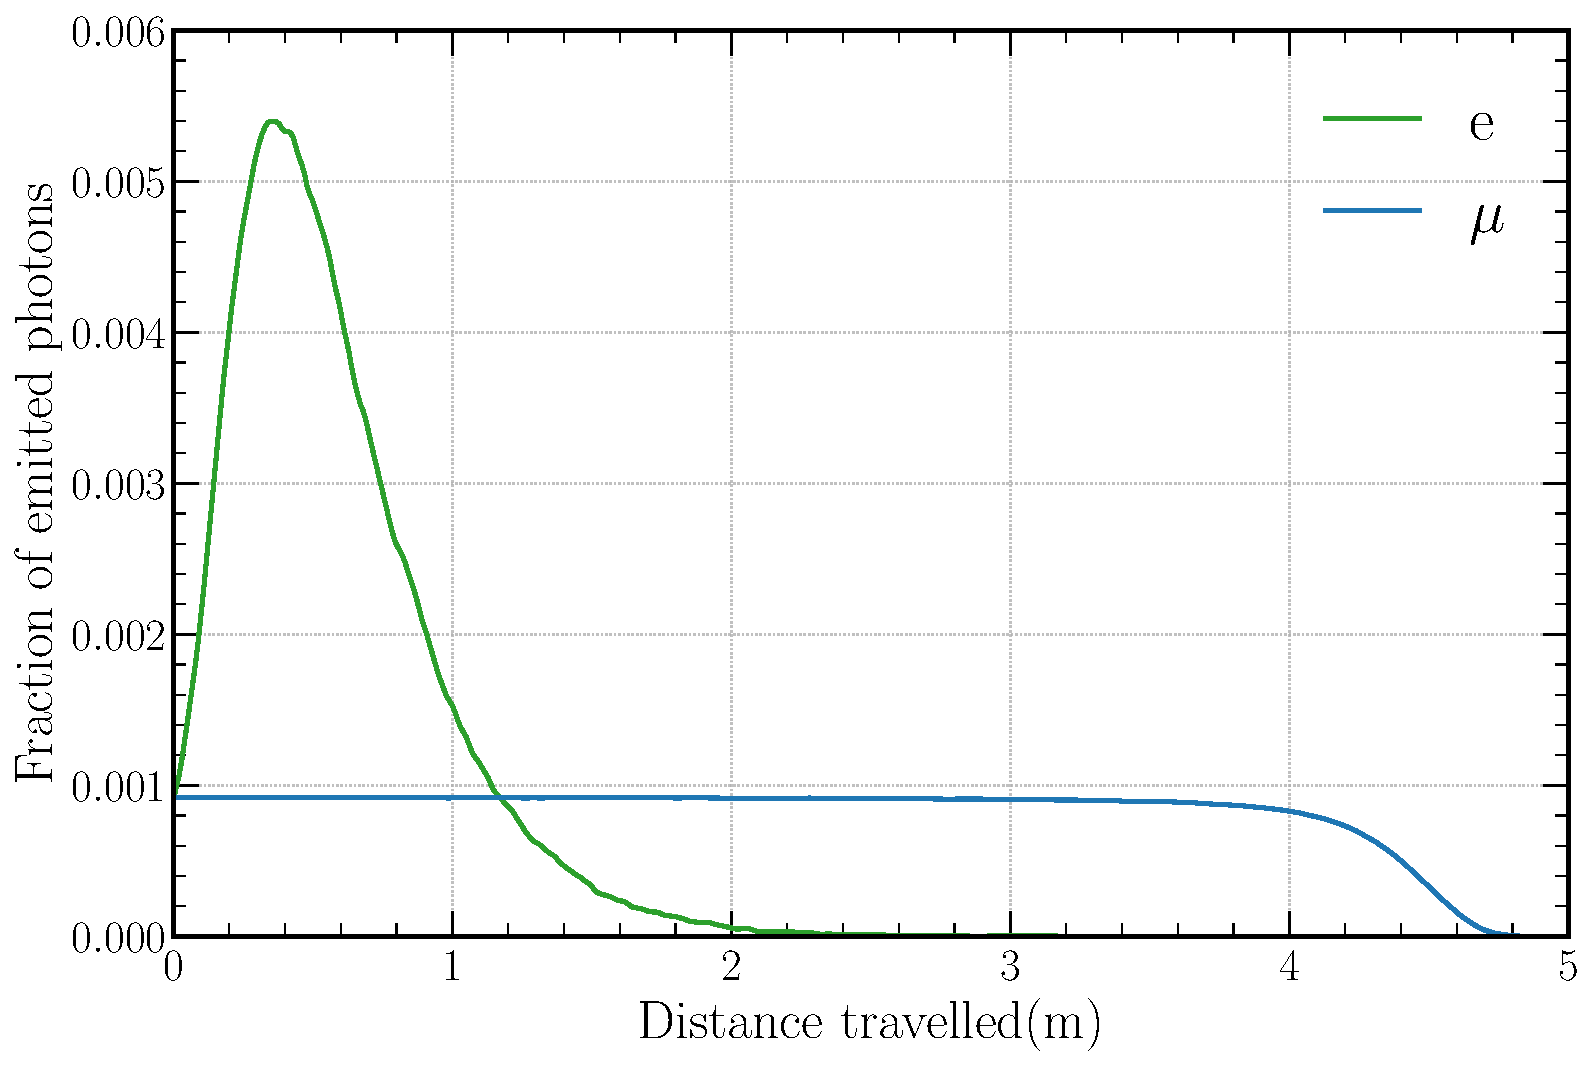
\includegraphics[width=0.6\textwidth]{diagrams/4-chips/emission_distance.pdf}
    \caption[Fraction of Cherenkov photons emitted as a function of distance]
    {Fraction of the total number of Cherenkov photons emitted as a function of the distance from
        the interaction vertex for both electrons and muons with an initial energy of
        \unit{2.5}{\GeV}. Multiple particles within the electron-induced electromagnetic shower
        emit their Cherenkov radiation over a short distance and in slightly different directions
        (fuzzy). Conversely, a muon travels relatively much further emitting an approximately
        constant level of Cherenkov radiation as it does so (clean).}
    \label{fig:emission distance}
\end{figure}

The situation quickly becomes complicated when multiple charged particles above the Cherenkov
threshold are involved, which is common at multi-$\GeV$ energies. In this case, multiple
overlapping rings are observed, making reconstruction difficult. The worst-case scenario is when
two rings overlap entirely, removing any ability to tell them apart. This topology is often the
case for NC interactions producing a $\pi^{0}$ in the final state, forming the primary background
for the signal CC $\nu_{e}$ appearance channel.

$\pi^{0}$ particles decay to a pair of photons with a 98.82\% branching ratio, both which almost
immediately initiate an electromagnetic shower, just like an electron~\cite{particle2020}. The
process leads to the formation of two electron like rings separated by an angle given by
\begin{equation}
    (1-\cos\theta_{ij})=\frac{m_{\pi}^2}{2E_{i}E_{k}},
\end{equation}
where $m_{\pi}$ is the invariant mass of the $\pi^{0}$ and $E_{i}$ and $E_{j}$ are the energies of
the two photons respectively. Therefore, for a $\pi^{0}$ decaying to two \unit{1}{\GeV} photons,
there is just $8^{\circ}$ of separation between the rings, making them difficult to tell apart.
This distinction is especially hard when electron like rings are also fuzzy. Alternatively, if the
two photons have an unequal energy distribution, such that one is much more energetic than the
other, the higher energy photon ring can dominate, and the other can not be identified, leading to
what looks like a single electron ring, producing a misidentification.

\section{The CHIPS-5 detector} %%%%%%%%%%%%%%%%%%%%%%%%%%%%%%%%%%%%%%%%%%%%%%%%%%%%%%%%%%%%%%%%%%%
\label{sec:chips_detector} %%%%%%%%%%%%%%%%%%%%%%%%%%%%%%%%%%%%%%%%%%%%%%%%%%%%%%%%%%%%%%%%%%%%%%%

\chipsfive is the first large scale prototype detector module for the \chips project. At
\unit{25}{\text{m}} wide and \unit{12}{\text{m}} high, \chipsfive is cylindrical in shape with an
inner surface area of \unit{1924}{\text{m}^2} and a total target mass of \unit{5.9}{\text{kton}}.
Via the process of design, construction, deployment, and data taking, \chipsfive primarily aims to
refine the \chips concept for future full-scale ($\sim$\unit{15}{\text{kton}}) modules.
Consequently, \chipsfive is designed such that the details outlined in this section are entirely
characteristic of what a full-sized \chips module is envisioned to be.

First, the location, structure, instrumentation, and water filtration are detailed for the
complete detector. A discussion of the construction and deployment procedure follows before the
current status is presented. The full electronics and DAQ details are given separately in
Chapter.~\ref{chap:daq}.

\subsection{Location} %%%%%%%%%%%%%%%%%%%%%%%%%%%%%%%%%%%%%%%%%%%%%%%%%%%%%%%%%%%%%%%%%%%%%%%%%%%%
\label{sec:chips_detector_location} %%%%%%%%%%%%%%%%%%%%%%%%%%%%%%%%%%%%%%%%%%%%%%%%%%%%%%%%%%%%%%

\chipsfive is located at the Wentworth 2W pit in northern Minnesota, USA, near the small town of
Hoyt Lakes. A disused and flooded surface Taconite ore (a type of iron ore) mine pit, Wentworth 2W
is located \unit{7}{\text{mrad}} off the \numi axis at a distance of \unit{712}{\text{km}} from
the beam target. Roughly \unit{0.8}{\text{km}} by \unit{1.2}{\text{km}} in size with a maximum
depth of \unit{60}{\text{m}} ($\pm$\unit{3}{\text{m}} throughout the year), the pit allows for a
water overburden of approximately \unit{50}{\text{m}} above \chipsfive when resting on the bottom.
With an average daily low temperate of $-24^{\circ}\text{C}$ in January, the pit freezes over
during winter, therefore, work is only possible during the summer months of May to October.

A sizeable earthen ramp on the south side of Wentworth 2W is used for detector construction. The
construction site is easily accessible by road and well connected to power due to the heavy
infrastructure in place for mining. Additionally, the nearby PolyMet mining administration
building is used as a laboratory environment for the construction and testing of individual
components before their installation within the detector. A labelled satellite view of Wentworth
2W is given in Fig.~\ref{fig:pit} for context, with an aerial picture of the construction site
shown in Fig.~\ref{fig:from_the_sky}.

\begin{figure} % PIT DIAGRAM %
    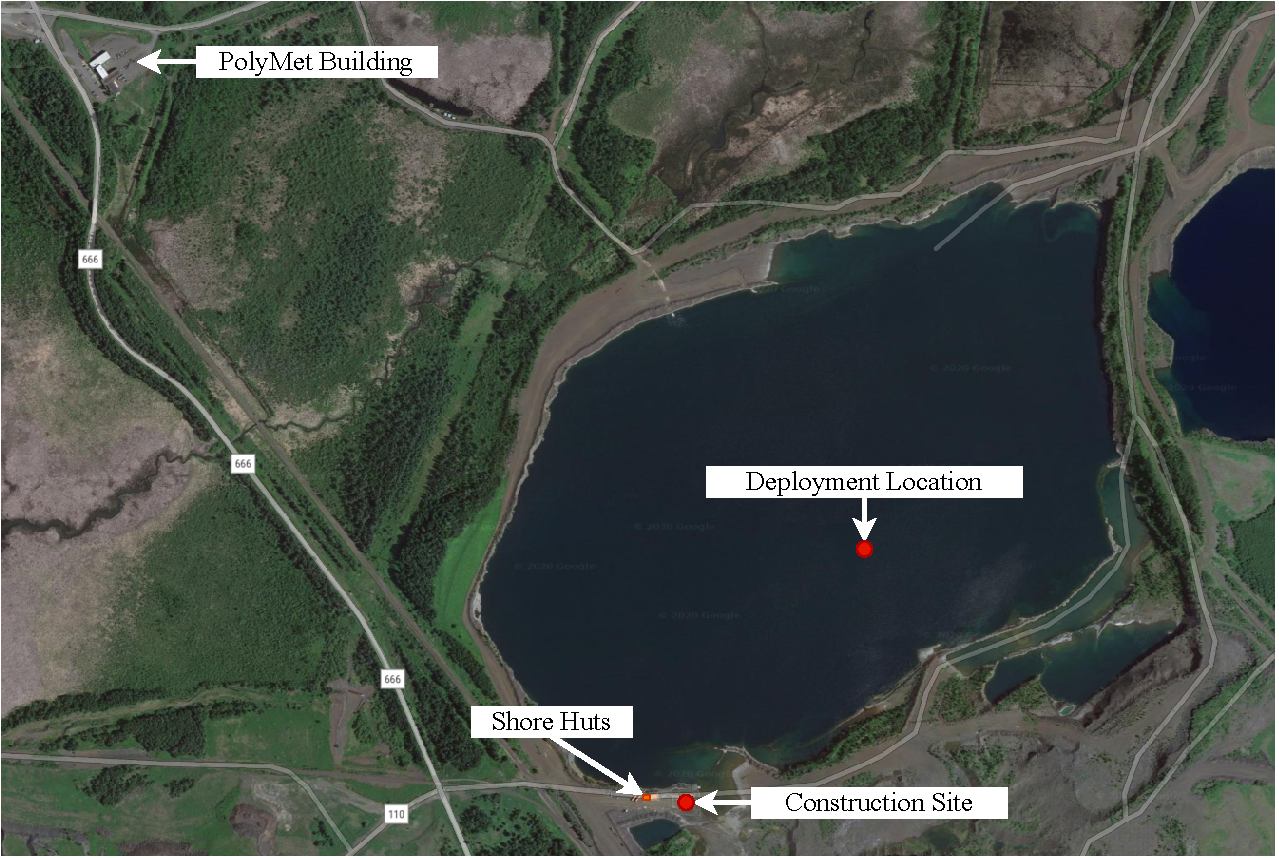
\includegraphics[width=\textwidth]{diagrams/4-chips/pit.pdf}
    \caption[Satellite view of the Wentworth 2W mine pit in northern Minnesota]
    {Satellite view of the Wentworth 2W flooded mine pit in northern Minnesota, showing key
        \chipsfive locations. The PolyMet building, shore huts, construction site, and deployment
        location are shown. For both the construction site and deployment location, the red circle
        shows the true \chipsfive detector size to scale.}
    \label{fig:pit}
\end{figure}

\begin{figure} % CHIPS FROM THE SKY DIAGRAM %
    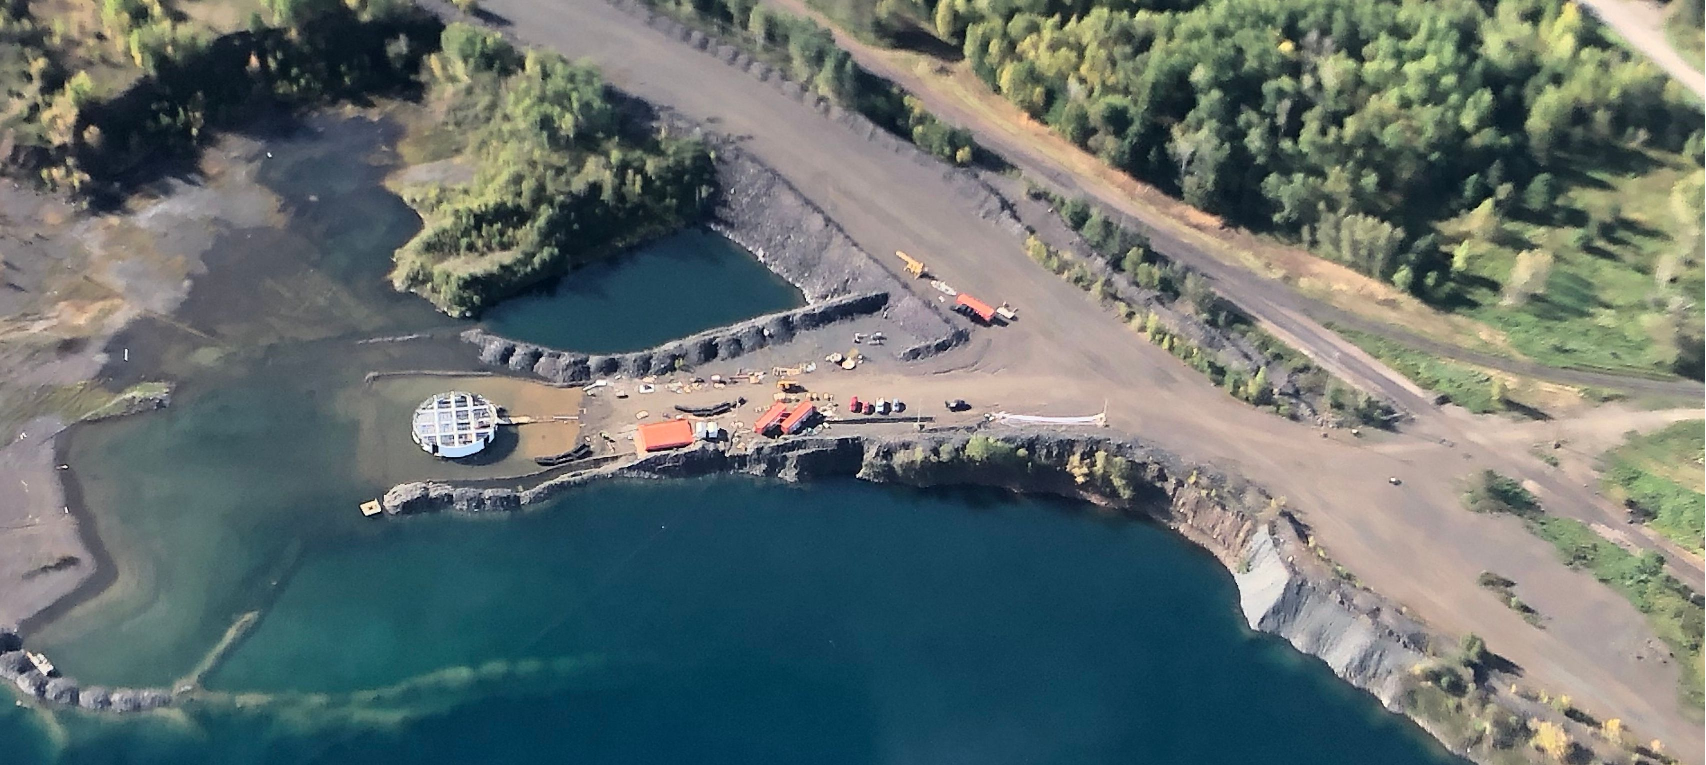
\includegraphics[width=\textwidth]{diagrams/4-chips/from_the_air.pdf}
    \caption[Aerial picture of the \chipsfive construction site]
    {Aerial picture of the \chipsfive construction site facing south. The Wentworth 2W pit is in
        the lower half of the image, with the part built \chipsfive detector visible at the bottom
        of the earthen construction ramp. The two white shore huts can be seen halfway up the
        ramp.}
    \label{fig:from_the_sky}
\end{figure}

\subsection{Structure} %%%%%%%%%%%%%%%%%%%%%%%%%%%%%%%%%%%%%%%%%%%%%%%%%%%%%%%%%%%%%%%%%%%%%%%%%%%
\label{sec:chips_detector_structure} %%%%%%%%%%%%%%%%%%%%%%%%%%%%%%%%%%%%%%%%%%%%%%%%%%%%%%%%%%%%%

The structure of the \chipsfive detector module consists primarily of two \unit{26}{\text{m}}
diameter and \unit{1.3}{\text{m}} high lightweight stainless steel circular \emph{endcaps} that
form the top and bottom of its cylindrical shape. During construction the conveniently named
\emph{top-cap} is held above the \emph{bottom-cap} by \unit{1.5}{\text{m}} long steel struts as
shown in Fig.~\ref{fig:frame}. This configuration allows for the endcap instrumentation, detailed
in Section.~\ref{sec:chips_detector_instrumentation}, to be easily installed.

\begin{figure} % CHIPS FRAME DIAGRAM %
    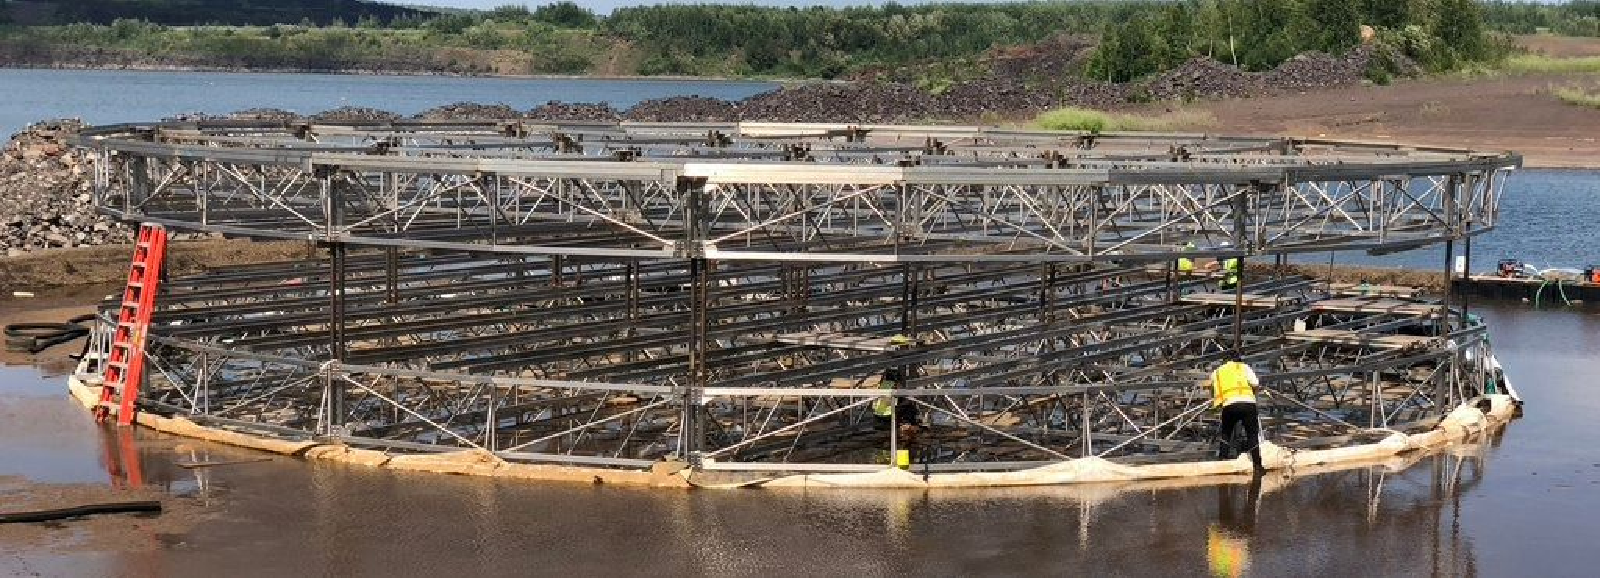
\includegraphics[width=\textwidth]{diagrams/4-chips/frame.pdf}
    \caption[Picture of the \chipsfive structural frame]
    {Picture of the \chipsfive structural frame with humans for scale. The endcaps can be seen
        separated by steel struts. Rows of stainless steel \emph{stringers} are attached to the
        inside of each endcap for instrumentation mounting.}
    \label{fig:frame}
\end{figure}

The two endcaps are connected by 28 Dyneema cables attached around their perimeter, each
\unit{12}{\text{m}} in length. Additionally, a total of 48 air-filled Polyvinyl Chloride (PVC)
pipes, each \unit{16}{\text{inches}} in diameter, are attached to the frame of the top-cap to make
it buoyant. Once deployed into the pit, the bottom-cap sinks while the top-cap floats, pulling the
Dyneema cable taut and forming the final expanded detector shape shown in
Fig.~\ref{fig:chips_render}.

\begin{figure} % CHIPS RENDER DIAGRAM %
    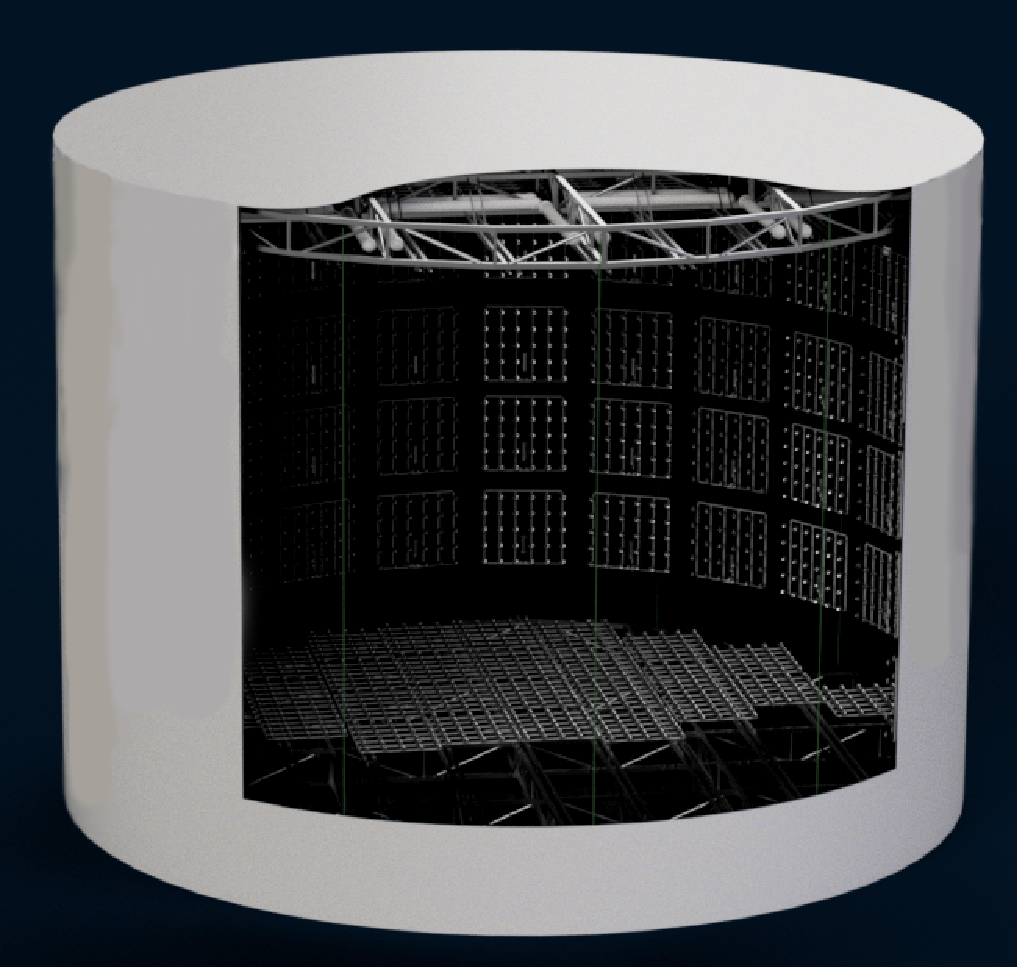
\includegraphics[width=0.6\textwidth]{diagrams/4-chips/chips_render.pdf}
    \caption[Graphical rendering of the \chipsfive detector]
    {Graphical rendering of the fully deployed and expanded \chipsfive detector module with a
        section of the liner cutaway. The bottom endcap and wall \textsc{Pom}s are visible, as
        well as the top endcap structure and floatation. The green lines indicate the Dyneema
        cables holding the endcaps together.}
    \label{fig:chips_render}
\end{figure}

A lightproof and watertight liner is also installed to surround the fully expanded structure.
Designed to isolate the clean internal water from the external pit water and to prevent
non-Cherenkov light from reaching the \PMTs, the liner is made from \emph{geomembrane}, a flexible
reinforced polymer membrane. Commercially available in large rolls, the liner is welded together
during construction to form the top, bottom, and sides. Note that when fully deployed, the liner
does not take any of the structural strain.

\subsection{Instrumentation} %%%%%%%%%%%%%%%%%%%%%%%%%%%%%%%%%%%%%%%%%%%%%%%%%%%%%%%%%%%%%%%%%%%%%
\label{sec:chips_detector_instrumentation} %%%%%%%%%%%%%%%%%%%%%%%%%%%%%%%%%%%%%%%%%%%%%%%%%%%%%%%

\chipsfive is instrumented with PMTs arranged within distinct plane like structures called Planar
Optical Modules (\textsc{Pom}s), which take inspiration from the Digital Optical Modules
(\textsc{Dom}s) used by IceCube and KM3NeT~\cite{hanson2006, eijk2015}. Each \textsc{Pom} is a
roughly \unit{2}{\text{m}} by \unit{3}{\text{m}} array of watertight PVC tubing equipped with
between $15$ to $30$ PMTs, as well as the lowest level of DAQ electronics. Commercially available
PVC piping and connectors are used to form the structure of each plane, glued together with
standard PVC primer and cement.

There are two types of \textsc{Pom} used within \chipsfive, differentiated by the PMTs and DAQ
electronics they use and named after the institution at which they were primarily developed.
Firstly, \emph{Nikhef} \textsc{Pom}s use \unit{88}{\text{mm}} wide HZC PMTs~\cite{hzc}, with
electronics developed for the KM3NeT experiment~\cite{katz2009, adrian2016}. Secondly,
\emph{Madison} \textsc{Pom}s use \unit{3}{\text{inch}} wide Hamamatsu PMTs~\cite{hamamatsu}, with
electronics developed by \chips in collaboration with the Wisconsin IceCube Particle Astrophysics
Centre (WIPAC) in Madison, Wisconsin.

The HZC PMTs have a high ratio of output electrons to incident photons (quantum efficiency) of
24.4\% at a wavelength of \unit{400}{\text{nm}}, compared to the low 12.0\% ratio achieved by the
Hamamatsu PMTs. Furthermore, the photon hit time resolution is $\sim$\unit{2}{\text{ns}} and
$\sim$\unit{5}{\text{ns}} for the HZC and Hamamatsu PMTs respectively.

In total $6114$ HZC, and $450$ Hamamatsu PMTs are arranged into $226$ Nikhef and $30$ Madison
\textsc{Pom}s respectively. Every PMT is housed within an assembly as shown in
Fig.~\ref{fig:nikhef_pmt_assembly} for the Nikhef case and Fig.~\ref{fig:madison_pmt_assembly} for
the Madison case. Importantly, to increase the level of light collection, each Nikhef PMT is
equipped with a \emph{light-cone} consisting of a circular reflective surface at \unit{45}{^\circ}
to the PMT normal. The Madison PMT assembly is similar but has no light-cone. For \textsc{Pom}s
attached to either endcap, their PMTs are angled at \unit{45}{^\circ} facing the direction of the
beam to optimise light collection.

All PMTs within a \textsc{Pom} are connected to the lowest level of DAQ electronics contained
within a dedicated onboard electronics box. Either an aluminium or PVC cylinder in the Nikhef or
Madison case respectively. A flexible PVC \emph{pigtail} is attached to each \textsc{Pom}
electronics box containing connections to the higher level DAQ and power supply. A
\emph{water-block} within each pigtail ensures that if either the external link or \textsc{Pom}
becomes flooded, the other is still capable of withstanding the \unit{6}{\text{atm}} of water
pressure at the bottom of the pit. A fully assembled and installed Nikhef \textsc{Pom} is shown in
Fig.~\ref{fig:single_plane} for reference.

\begin{figure} % NIKHEF PMT ASSEMBLY DIAGRAM %
    \centering
    \subcaptionbox{Disassembled}{%
        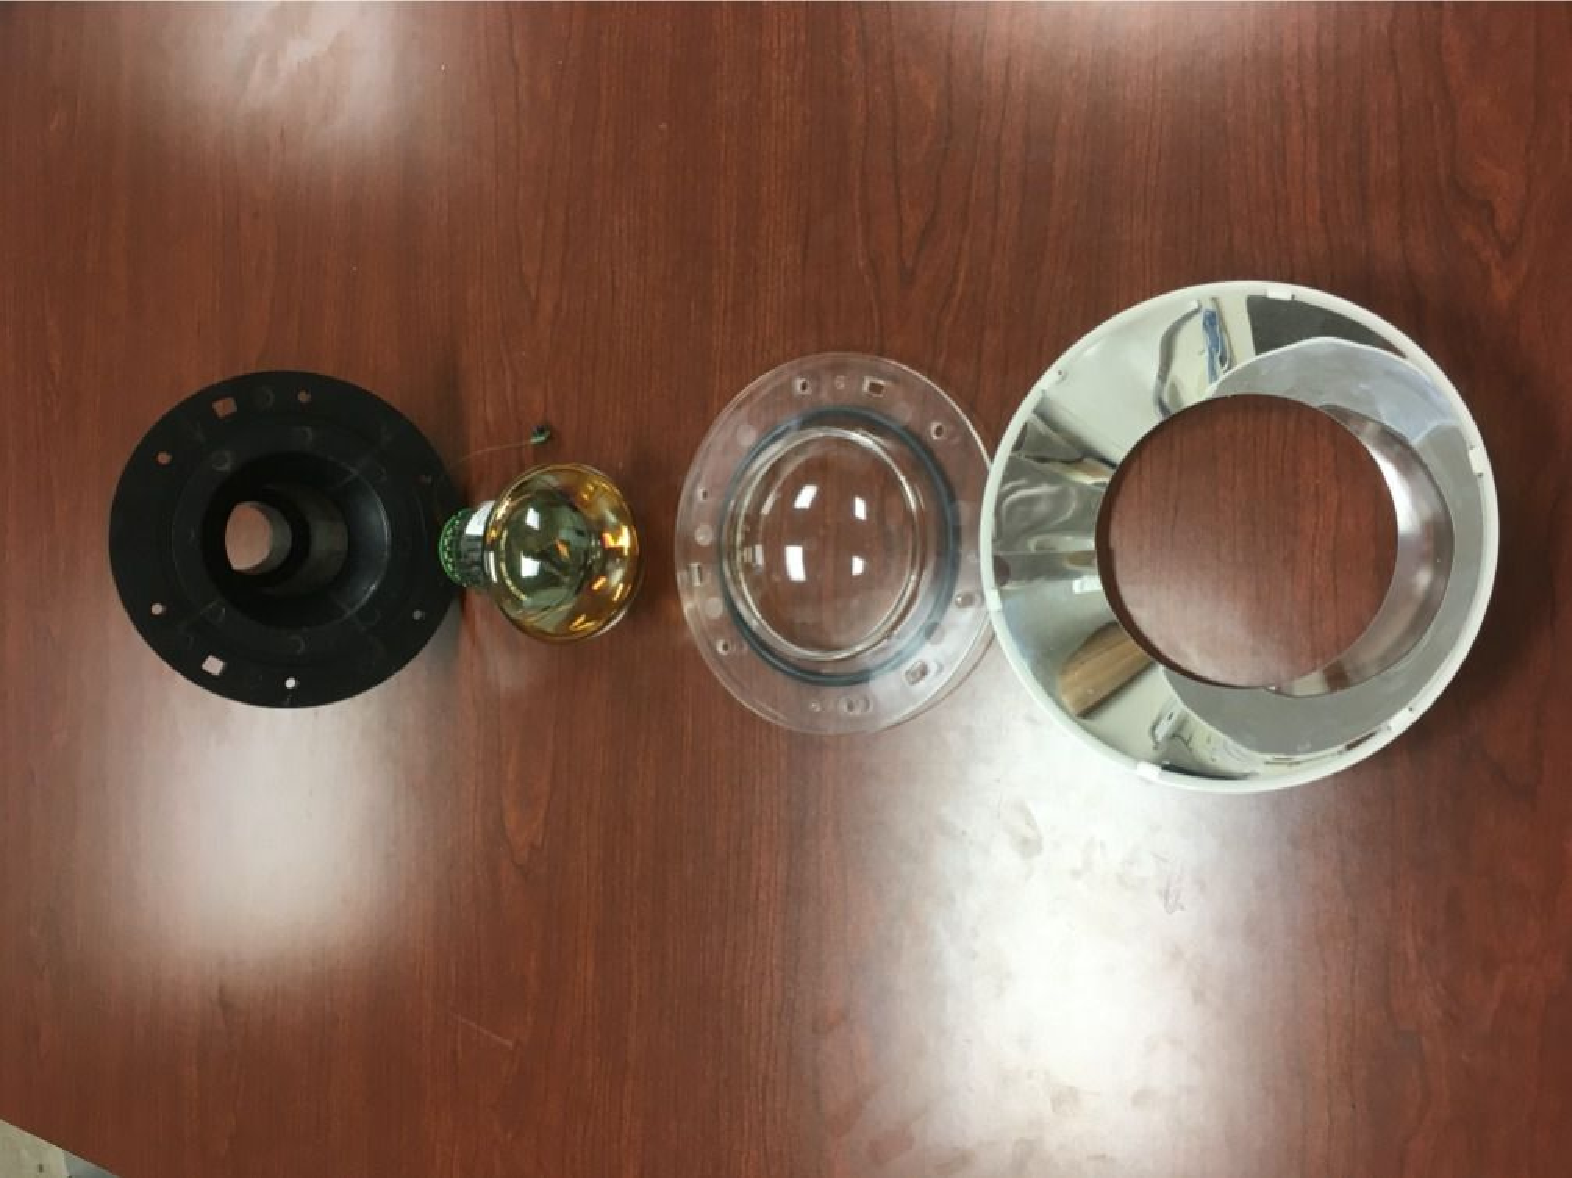
\includegraphics[height=5.5cm]{diagrams/4-chips/pmt_disassembled.pdf}%
    }
    \quad
    \subcaptionbox{Assembled}{%
        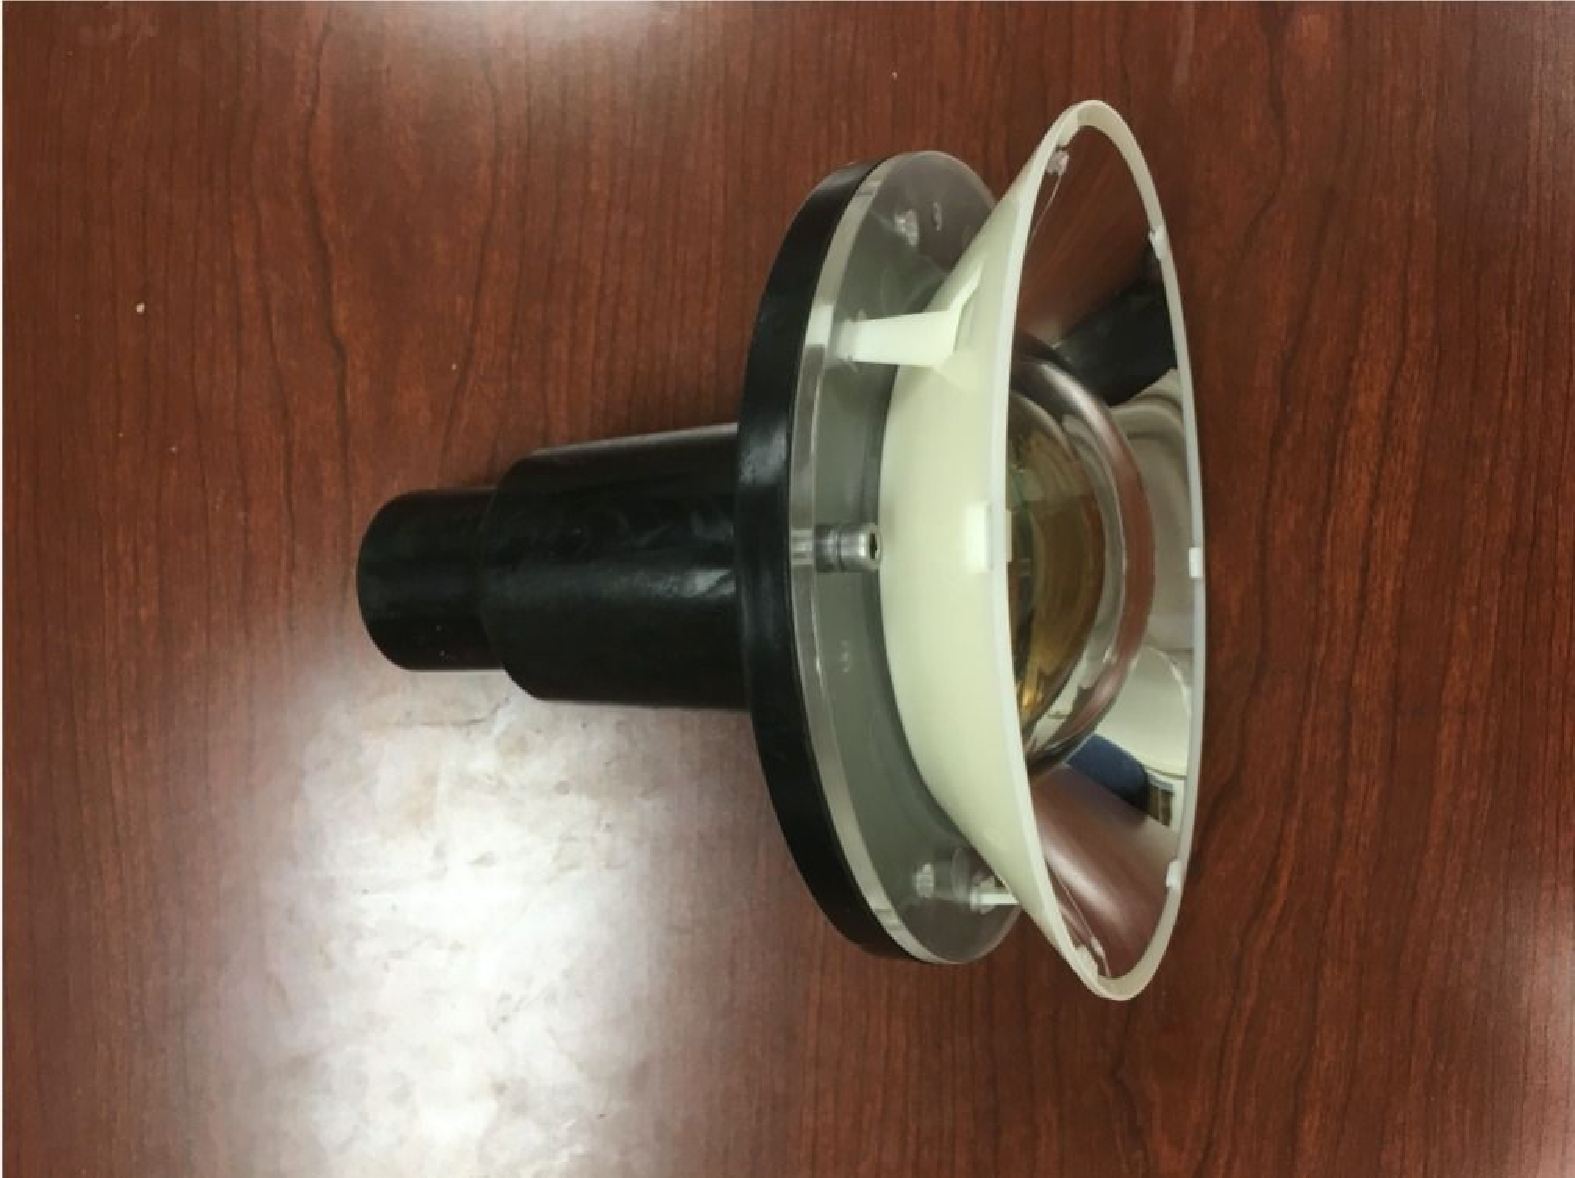
\includegraphics[height=5.5cm]{diagrams/4-chips/pmt_assembled.pdf}%
    }
    \caption[Disassembled and assembled Nikhef PMT housing components]
    {Disassembled (a) and assembled (b) Nikhef PMT assembly components. The assembly comprises of
        a black PVC insert, a HZC PMT, a transparent acrylic cover, and a reflective light-cone.
        The PMT is glued to the inside surface of the cover using a silicone-based optical gel,
        and a watertight seal is made between the insert and cover using an O-ring. The reflective
        light-cone is clipped to the front of the cover, and the whole assembly is glued into the
        \textsc{Pom} PVC structure.}
    \label{fig:nikhef_pmt_assembly}
\end{figure}

\begin{figure} % MADISON PMT ASSEMBLY DIAGRAM %
    \centering
    \subcaptionbox{Outside}{%
        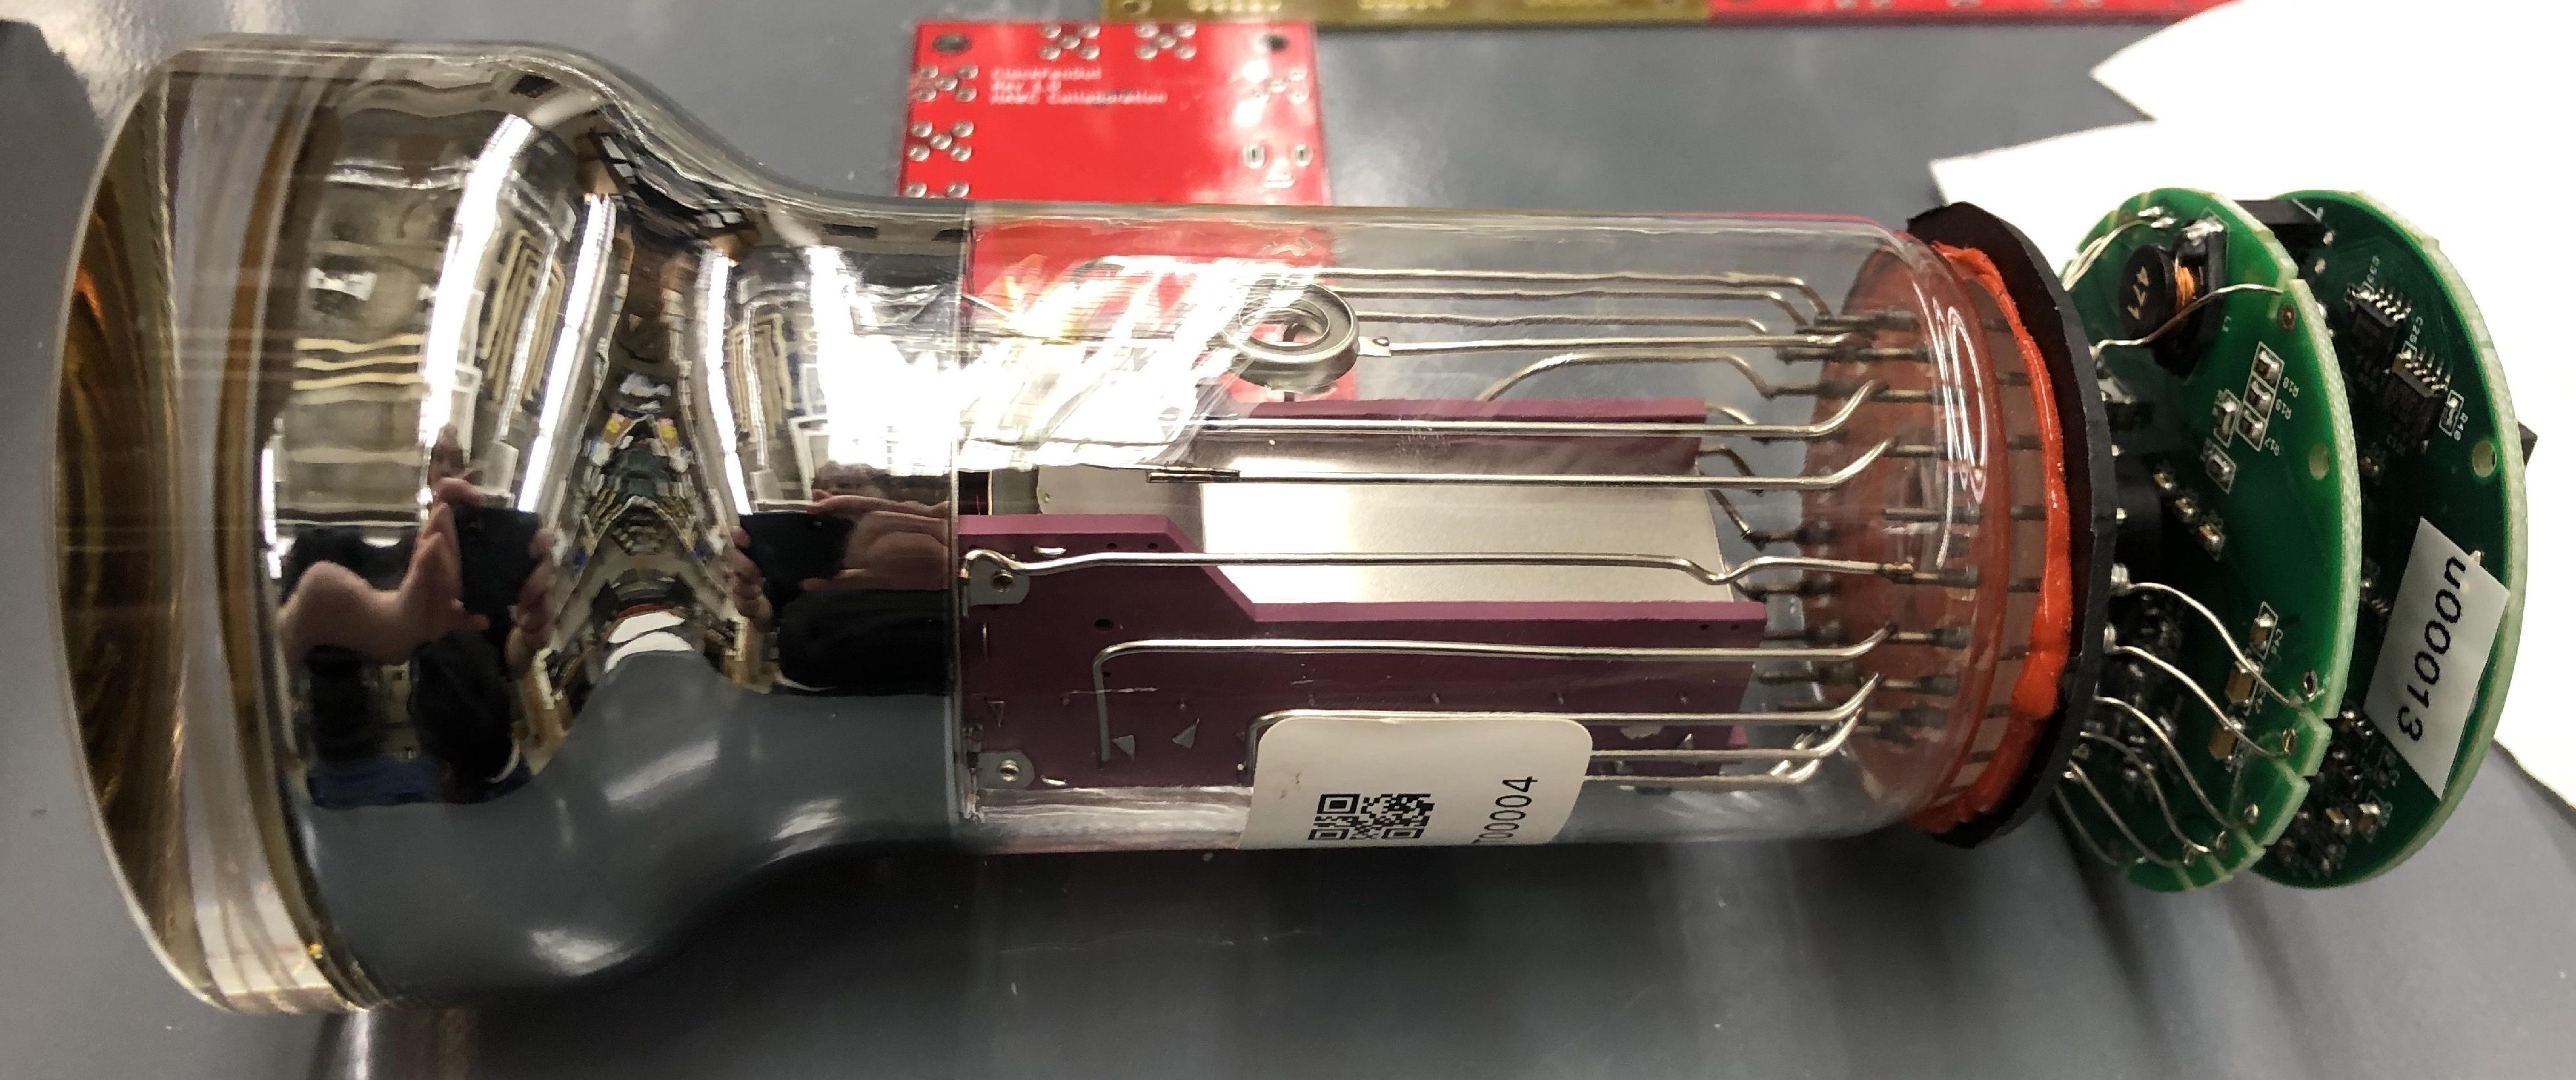
\includegraphics[angle=270,origin=c,height=4.3cm]{diagrams/4-chips/madison_pmt.pdf}%
    }
    \quad
    \subcaptionbox{Inside}{%
        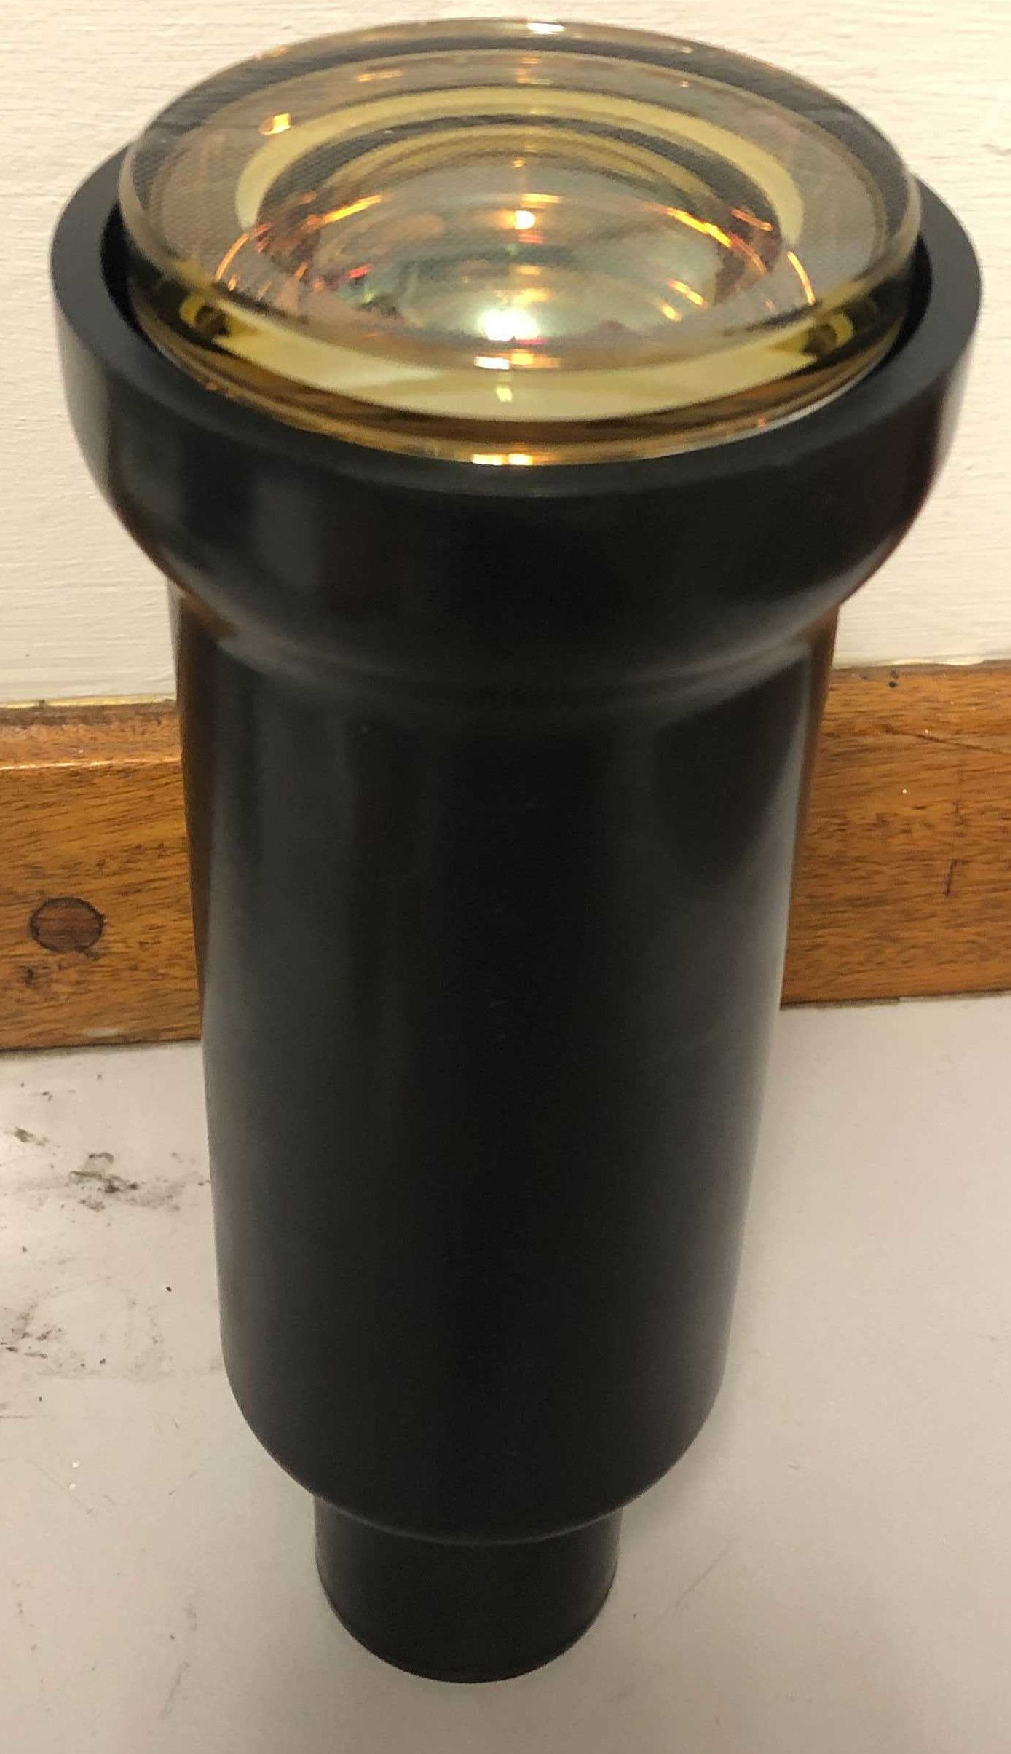
\includegraphics[height=6cm]{diagrams/4-chips/madison_assembly.pdf}%
    }
    \caption[Pictures of the Madison PMT assembly]
    {A Hamamatsu PMT outside (a) and inside its insert (b). The PMT is potted inside its black PVC
        insert to create a watertight seal that can withstand the \unit{6}{\text{atm}} of water
        pressure at the bottom of the pit. A $\micro$DAQ detailed in Chapter.~\ref{chap:daq}, is
        seen attached to the base of the PMT in (a).}
    \label{fig:madison_pmt_assembly}
\end{figure}

\begin{figure} % NIKHEF \textsc{Pom} DIAGRAM %
    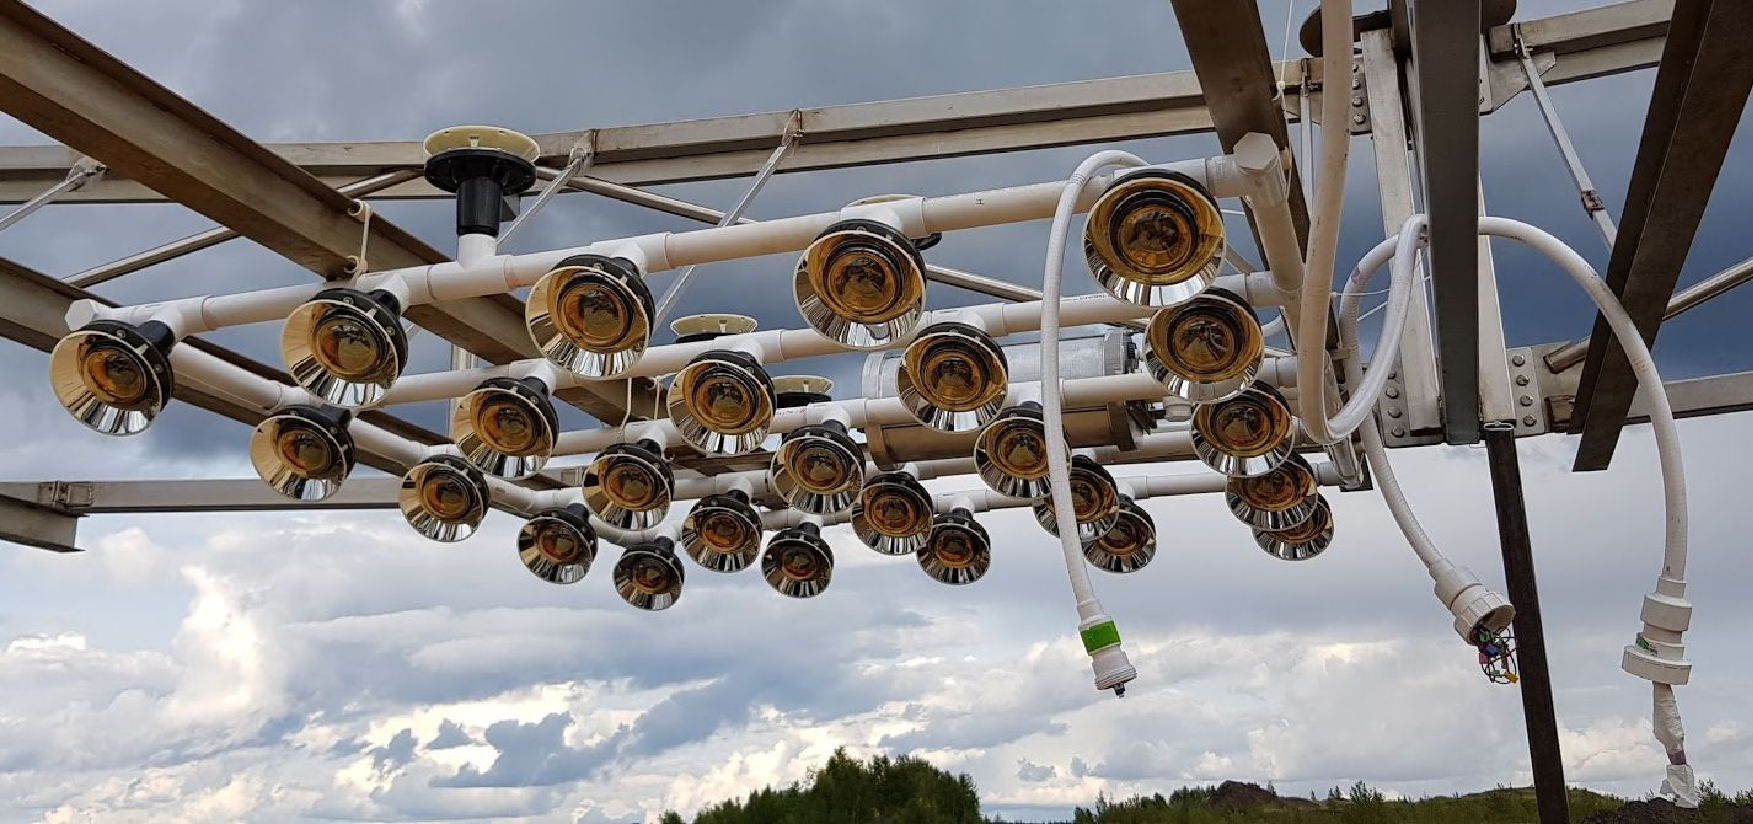
\includegraphics[width=\textwidth]{diagrams/4-chips/single_plane.pdf}
    \caption[Picture of a Nikhef \textsc{Pom}]
    {Picture of a single Nikhef full-density \textsc{Pom} installed on the top-cap of the
        \chipsfive detector. Both the inward-facing and veto PMTs are visible as well as the
        aluminium electronics container and pigtail, whose end is covered in green tape.}
    \label{fig:single_plane}
\end{figure}

The \textsc{Pom}s are tiled next to each other on the detector walls, attached to either the
stainless steel stringers on the top-cap and bottom-cap, or clipped to the Dyneema cables on the
vertical walls of the \emph{barrel}. As mentioned previously, full high density detector
instrumentation is not required for \chips detector modules, for two main reasons.

Firstly, only highly directional accelerator beam events are to be studied. Therefore, the vast
majority of neutrino interaction Cherenkov radiation is deposited on a relatively small downstream
region of the detector walls. Secondly, beam neutrinos predominantly have multi-$\GeV$ energies,
yielding a relatively large amount of Cherenkov radiation. Therefore, a smaller number of PMTs are
required to capture adequate Cherenkov radiation from each interaction.

Consequently, the distribution of the percentage of the detector walls covered by sensitive PMT
surface area (\emph{photocathode coverage}) is optimised within \chipsfive to reduce the total
number of PMTs used. The detector is split into three distinct regions of PMT photocathode
coverage whose boundaries are defined by their azimuth angle $\phi$ from the centre of the
downstream wall (where $\phi=0^{\circ}$) using the centre of the detector as the origin. Each
boundary is chosen by inspecting the fraction of beam Cherenkov photons that hit the detector
walls as a function of $\phi$. This distribution, generated by the detector simulation (outlined
in Section.~\ref{sec:chips_monte_carlo_sim}), is shown in Fig.~\ref{fig:coverage} alongside the
chosen boundaries.

\begin{figure} % COVERAGE DIAGRAM %
    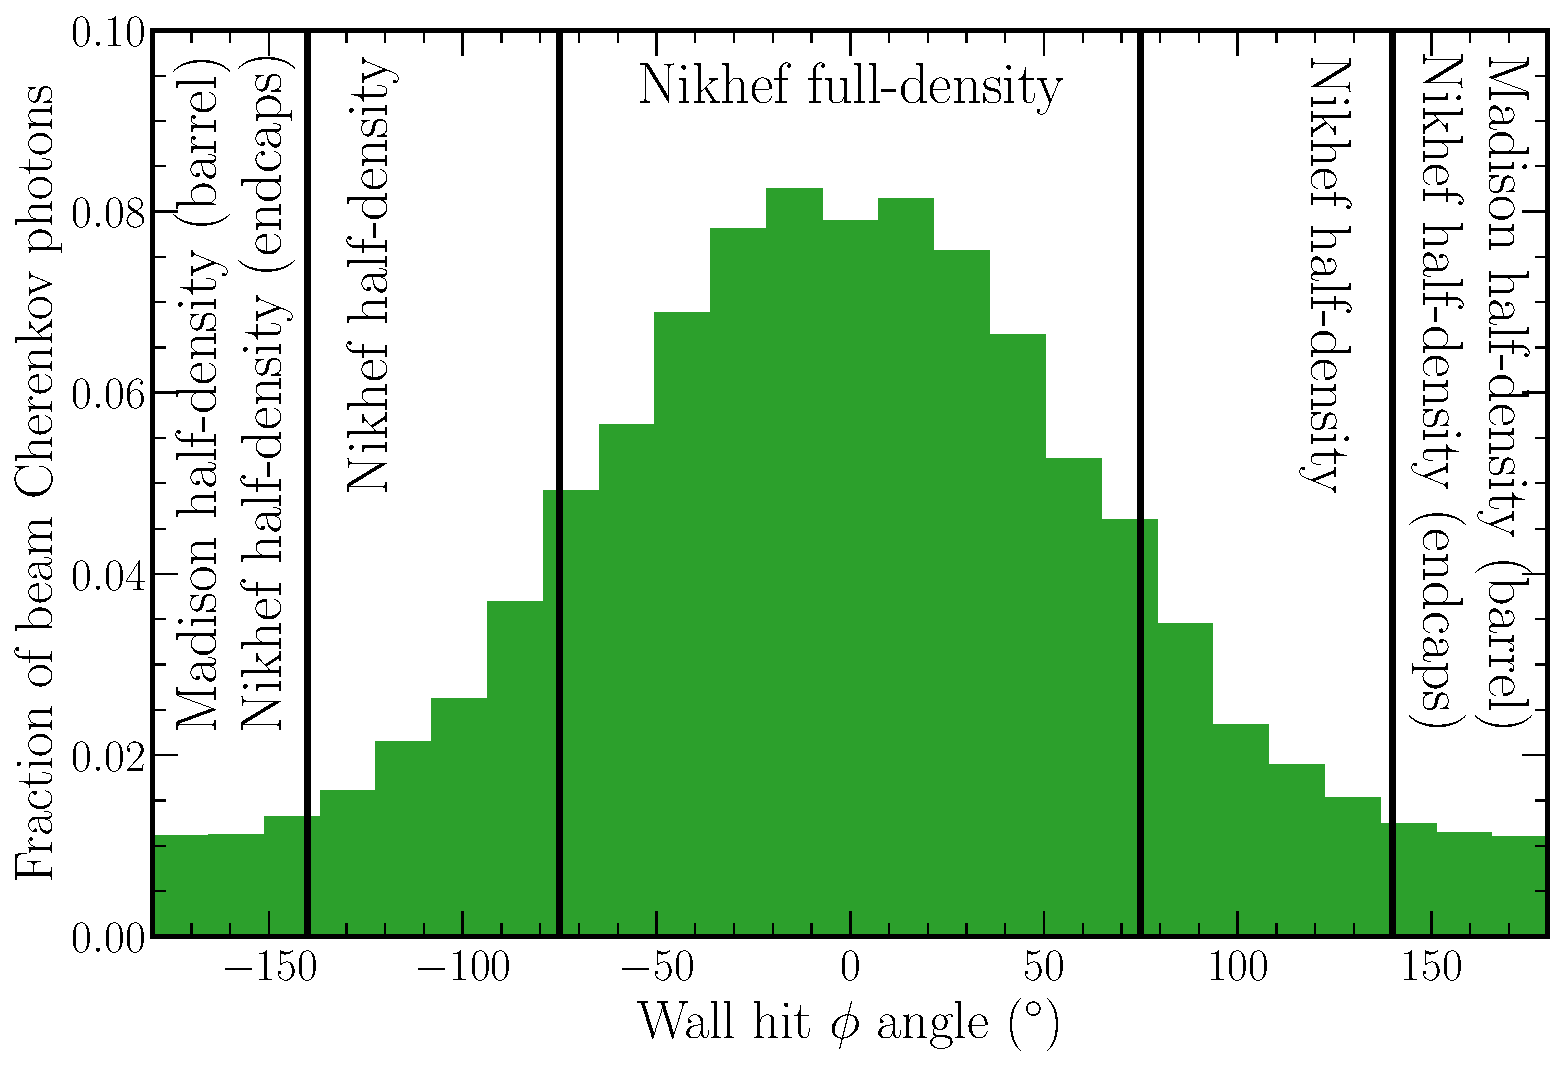
\includegraphics[width=0.8\textwidth]{diagrams/4-chips/coverage.pdf}
    \caption[Fraction of beam event Cherenkov photons that hit the detector walls as a function of
        the hit angle] {Fraction of beam event Cherenkov photons that hit the detector walls as a
        function of the hit angle $\phi$. The different photocathode coverage regions are
        indicated.}
    \label{fig:coverage}
\end{figure}

Firstly, there is a \emph{full-density} Nikhef \textsc{Pom} region in the most downstream
$\phi=\pm75^{\circ}$ region of the detector with a $\sim3\%$ photocathode coverage. Secondly, a
\emph{half-density} Nihkef \textsc{Pom} region covering the $\phi=\pm75^{\circ}$ to
$\phi=\pm180^{\circ}$ region of the endcaps and the $\phi=\pm75^{\circ}$ to $\phi=\pm140^{\circ}$
region of the barrel with a $\sim1.5\%$ photocathode coverage. Finally, a \emph{half-density}
Madison \textsc{Pom} region covering the $\phi=\pm140^{\circ}$ to $\phi=\pm180^{\circ}$ upstream
region of the barrel with a $\sim0.8\%$ photocathode coverage. Simulation studies have shown that
this configuration results in a negligible change in performance while vastly reducing the number
of required PMTs~\cite{blake2016}.

The \chipsfive detector module is equipped with a veto region within the top-cap frame structure
to aid cosmic muon rejection. Separated from the main detector volume by a geomembrane liner, the
\unit{1.3}{\text{m}} high region allows for the rejection of predominantly downward going cosmic
muons by detecting the Cherenkov radiation they produce. A total of $324$ upward-facing HZC veto
PMTs within the top-cap Nikhef \textsc{Pom}s give a veto photocathode coverage of $\sim0.6\%$. A
graphical rendering of the full top-cap instrumentation, showing the different density regions and
veto PMTs, is shown in Fig.~\ref{fig:top_cap}.

\begin{figure} % TOP CAP RENDER DIAGRAM %
    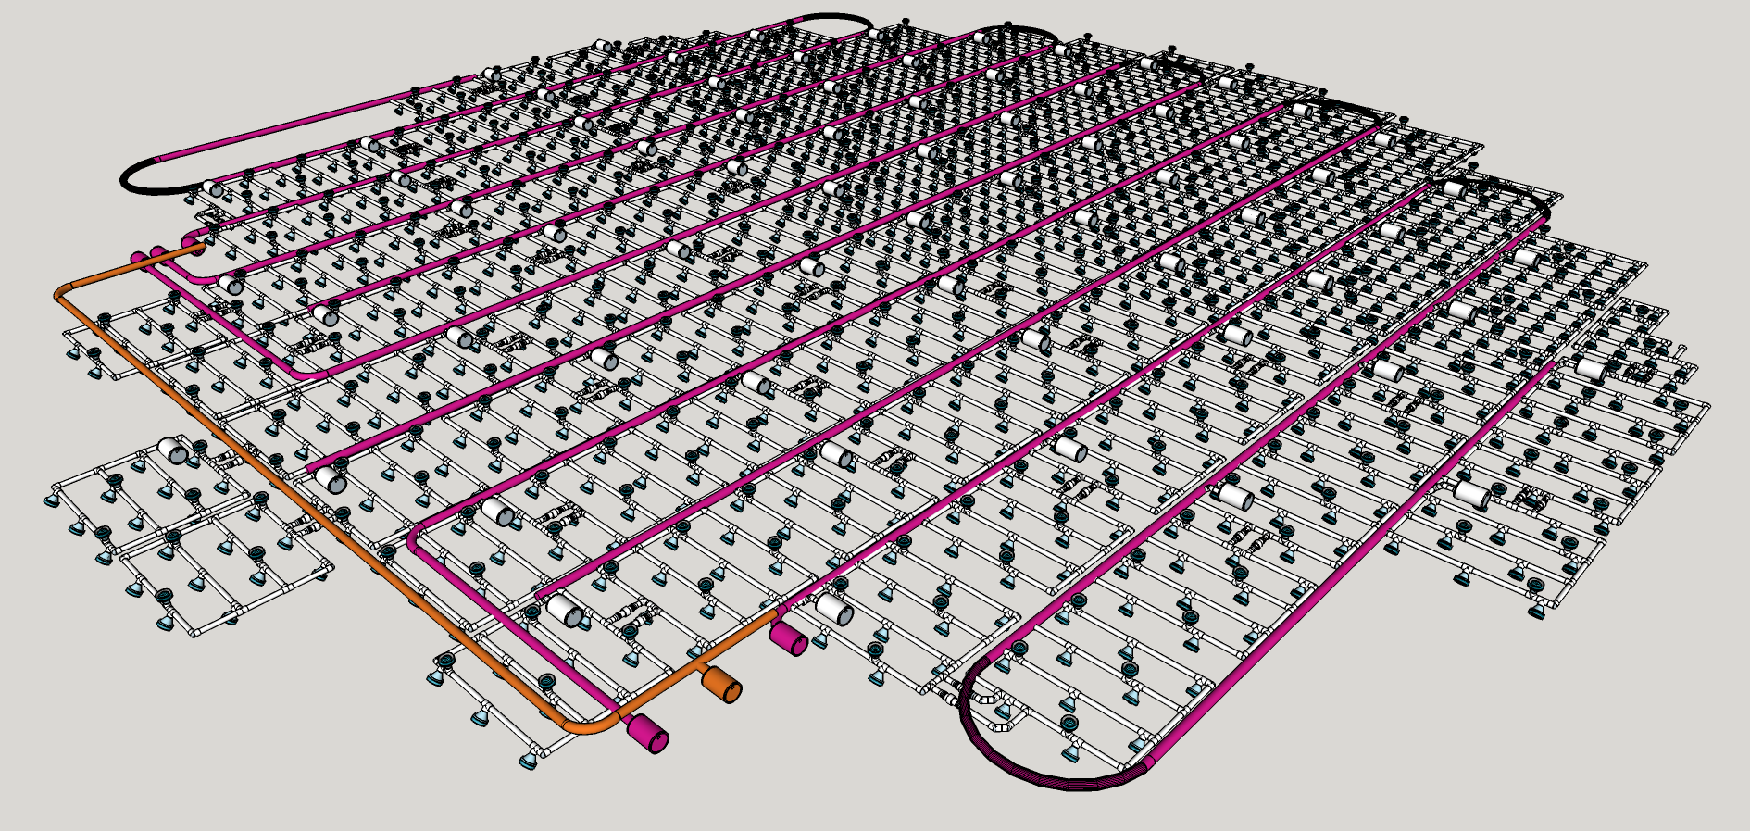
\includegraphics[width=\textwidth]{diagrams/4-chips/top_cap.pdf}
    \caption[Graphical rendering of the top-cap Planar Optical Modules]
    {Graphical rendering of the top-cap \textsc{Pom}s. Both the different photocathode coverage
        regions and the veto PMTs (contained within the top-cap \textsc{Pom}s) are visible. The
        \emph{manifolds} connecting the \textsc{Pom}s with the higher level DAQ components are
        also shown in pink and orange.}
    \label{fig:top_cap}
\end{figure}

All \chipsfive instrumentation receives power and is connected to the highest level DAQ systems
through a \unit{500}{\text{m}} long flexible PVC umbilical resting on the pit floor. The umbilical
contains a single optical fibre for data and two shielded gauge 10 cables for power. One end of
the umbilical is attached to the bottom-cap of the detector while the other enters a hut on shore
containing the master power supply and onshore DAQ equipment.

\subsection{Filtration} %%%%%%%%%%%%%%%%%%%%%%%%%%%%%%%%%%%%%%%%%%%%%%%%%%%%%%%%%%%%%%%%%%%%%%%%%%
\label{sec:chips_detector_water} %%%%%%%%%%%%%%%%%%%%%%%%%%%%%%%%%%%%%%%%%%%%%%%%%%%%%%%%%%%%%%%%%

Though surprisingly clear, the Wentworth 2W pit water requires filtration to reach the necessary
\unit{30}{\text{m}} photon attenuation length. Therefore, a high volume pump is used to
continually pull the internal detector water through a \unit{500}{\text{m}} long pipe to a
filtration hut on the shore. After filtration, the water is returned to the detector through a
second such pipe.

Within the hut, ten parallel sets of filters are installed in order to achieve a reasonable flow
rate, allowing for the full detector volume to be filtered every ten days. Each filter set
consists of a 20 inch \unit{10}{\micro\text{m}} carbon block filter followed by a 20 inch
\unit{0.5}{\micro\text{m}} polypropylene filter, as shown in fig.~\ref{fig:filtration}. This
configuration is found to achieve a photon attenuation length of \unit{133\pm2}{\text{m}} after
approximately two months of constant filtering~\cite{campbell2020}.

\begin{figure} % SIMULATION GEOM DIAGRAM %
    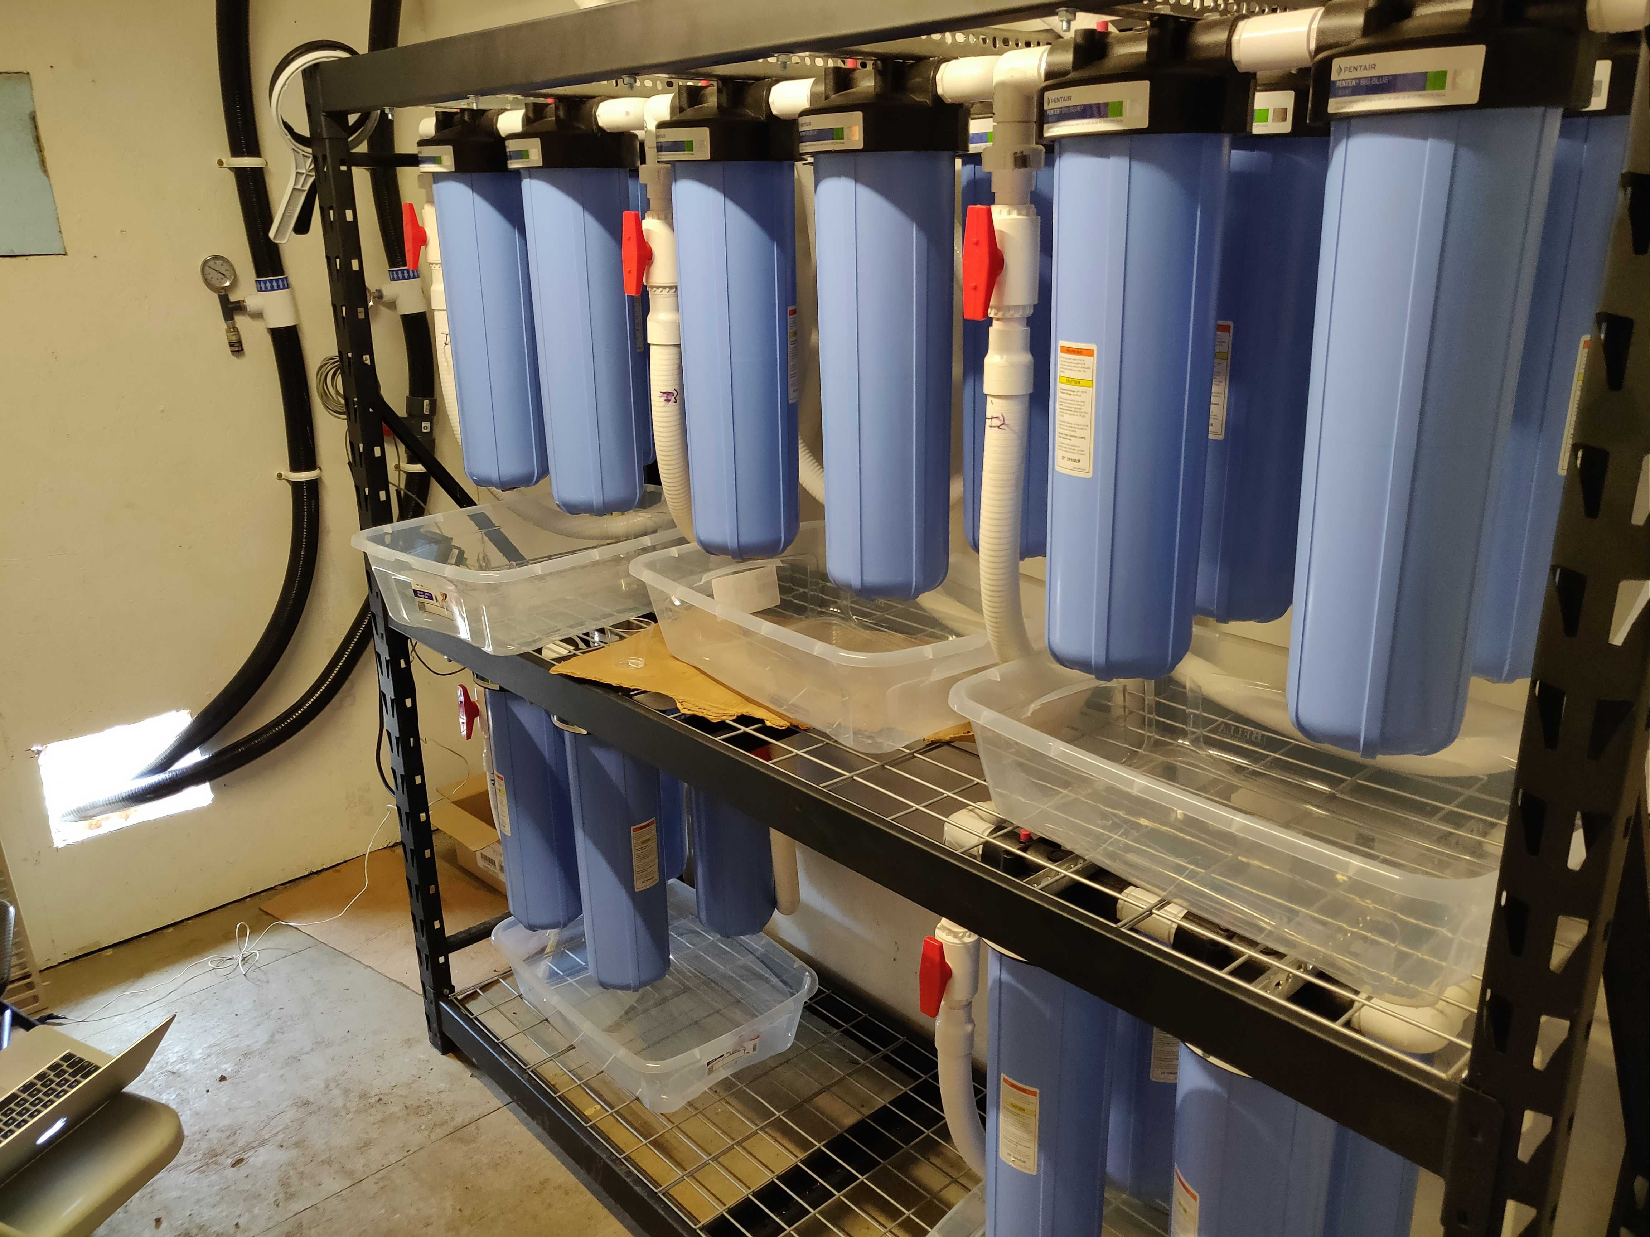
\includegraphics[width=0.6\textwidth]{diagrams/4-chips/filtration.pdf}
    \caption[Picture of the \chipsfive filtration system]
    {Picture of the \chipsfive filtration system within one of the shore huts. The pipes to and
        from the detector can be seen entering and exiting the hut respectively via a gap in the
        back wall.}
    \label{fig:filtration}
\end{figure}

\subsection{Construction and deployment} %%%%%%%%%%%%%%%%%%%%%%%%%%%%%%%%%%%%%%%%%%%%%%%%%%%%%%%%%
\label{sec:chips_detector_deployment} %%%%%%%%%%%%%%%%%%%%%%%%%%%%%%%%%%%%%%%%%%%%%%%%%%%%%%%%%%%%

The construction and deployment of any \chips detector module is a bespoke process that is
relatively complex when compared to other experiments. This complexity is primarily due to a body
of water being used for activities rather than solid ground. Below a simplified version of the
\chipsfive construction and deployment procedure is outlined.

\begin{enumerate}
    \item An earthen barrier is built separating the main body of Wentworth 2W from the
          construction area. As the pit water level rises during the summer, this acts as a dam
          preventing the construction area from flooding (at least in theory).
    \item The bottom-cap liner is welded together before the endcap structural frames are
          constructed above, resulting in that shown by Fig.~\ref{fig:frame}.
    \item The barrel liner is partly constructed starting from the detector base. Using a vertical
          liner roll for each of the 28 sides, the barrel liner is welded up to the height of the
          top-cap, as is shown in Fig.~\ref{fig:chips_with_liner}. The top-cap liner is also
          installed but not welded to the barrel liner.
    \item A strongly buoyant \emph{floating-dock}, made from steel and large plastic floats, is
          constructed surrounding the detector. The bottom-cap is attached with metal chains to
          winches on the floating-dock and with the Dyneema cables to winches on the top-cap.
    \item The pre-assembled and tested endcap \textsc{Pom}s are installed along with their
          associated power and data connections as well as other high-level DAQ components.
    \item The earthen barrier is removed and the construction area flooded, causing the detector
          and floating-dock structure to float. The detector is towed by a boat to its deployment
          location.
    \item The detector is slowly filled with water at the same time as being lowered using the
          winches on the floating-dock. This process continues until the top-cap reaches the
          surface of the water and begins the float. At this point, the steel struts separating
          the endcaps are removed.
    \item The barrel \textsc{Pom}s are installed in layers, brought to the detector location by
          boat. The gap between the barrel and top-cap liner allows this to happen. After a
          complete layer has been installed the bottom-cap is lowered using the winches on the
          floating-dock and top-cap and the barrel liner is correspondingly welded to a greater
          height before the procedure repeats.
    \item After all the \textsc{Pom}s have been installed, the barrel and top-cap liner are welded
          together, the detector umbilical attached, and the whole detector lowered until it rests
          at the bottom of the pit.
\end{enumerate}

\begin{figure} % CHIPS WITH LINER DIAGRAM %
    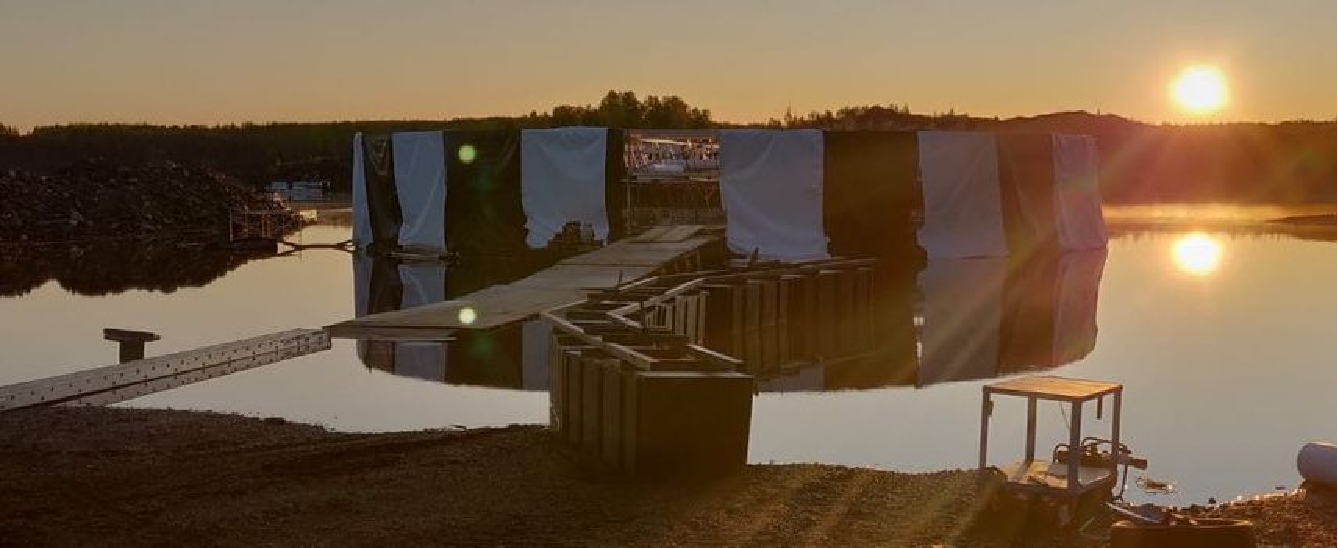
\includegraphics[width=\textwidth]{diagrams/4-chips/chips_with_liner_sun.pdf}
    \caption[Picture of the \chipsfive detector module with liner]
    {Picture of the \chipsfive detector module with liner welded up to the height of the top-cap.
        A section of the floating-dock can also be seen in the foreground.}
    \label{fig:chips_with_liner}
\end{figure}

\subsection{Current status} %%%%%%%%%%%%%%%%%%%%%%%%%%%%%%%%%%%%%%%%%%%%%%%%%%%%%%%%%%%%%%%%%%%%%%
\label{sec:chips_detector_status} %%%%%%%%%%%%%%%%%%%%%%%%%%%%%%%%%%%%%%%%%%%%%%%%%%%%%%%%%%%%%%%%

During the summer of 2018 and 2019 extensive \chipsfive construction work was carried out by a
team of 10 to 15 collaborators at any one time. Given the novel nature of the project, most tasks,
some of which are pictured in Fig.~\ref{fig:work1} and Fig.~\ref{fig:work2}, proved challenging
and time consuming.

\begin{figure} % WORK DIAGRAM 1 %
    \centering
    \subcaptionbox{Cornerstone placement.}{%
        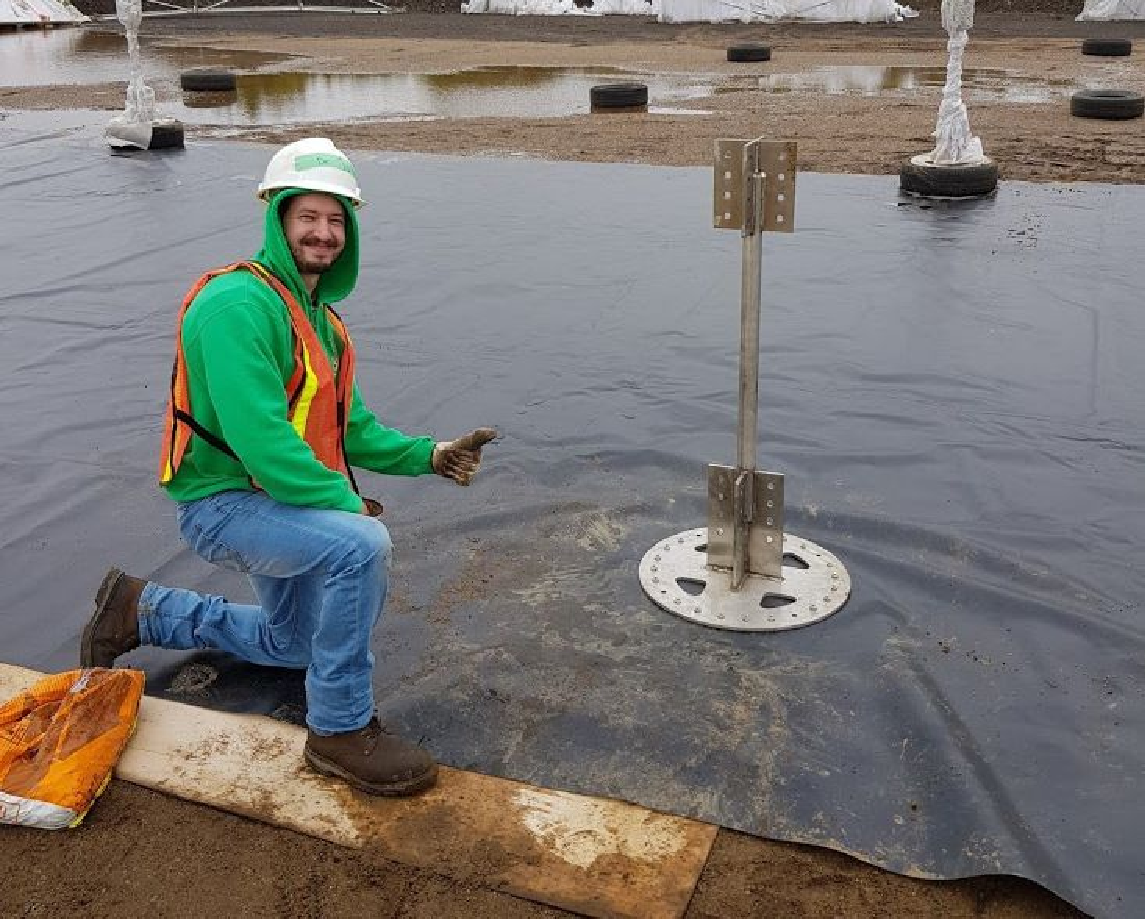
\includegraphics[height=6.5cm]{diagrams/4-chips/work2.pdf}%
    }
    \quad
    \subcaptionbox{Floatation production.}{%
        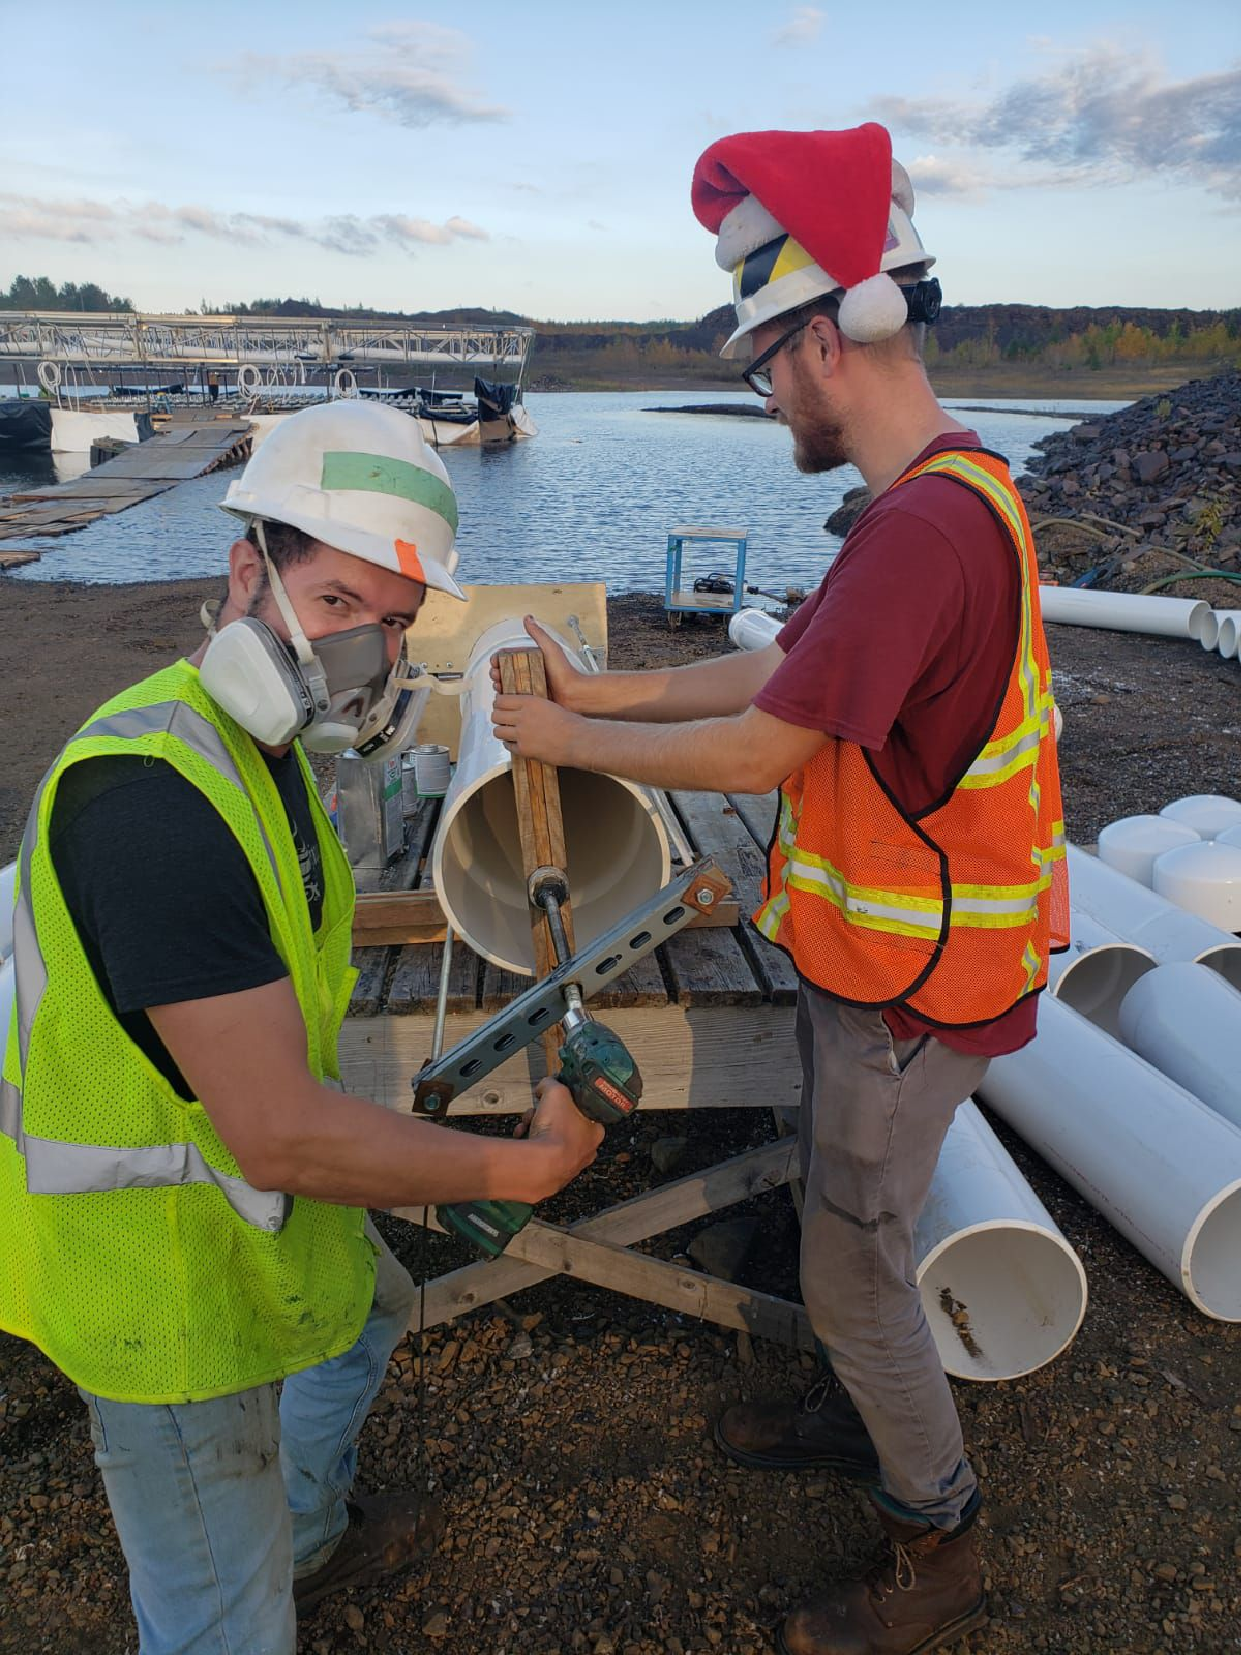
\includegraphics[height=6.5cm]{diagrams/4-chips/work3.pdf}%
    }
    \caption[Some \chipsfive construction work]
    {Some \chipsfive construction work.}
    \label{fig:work1}
\end{figure}

\begin{figure} % WORK DIAGRAM 2 %
    \centering
    \subcaptionbox{Connection testing.}{%
        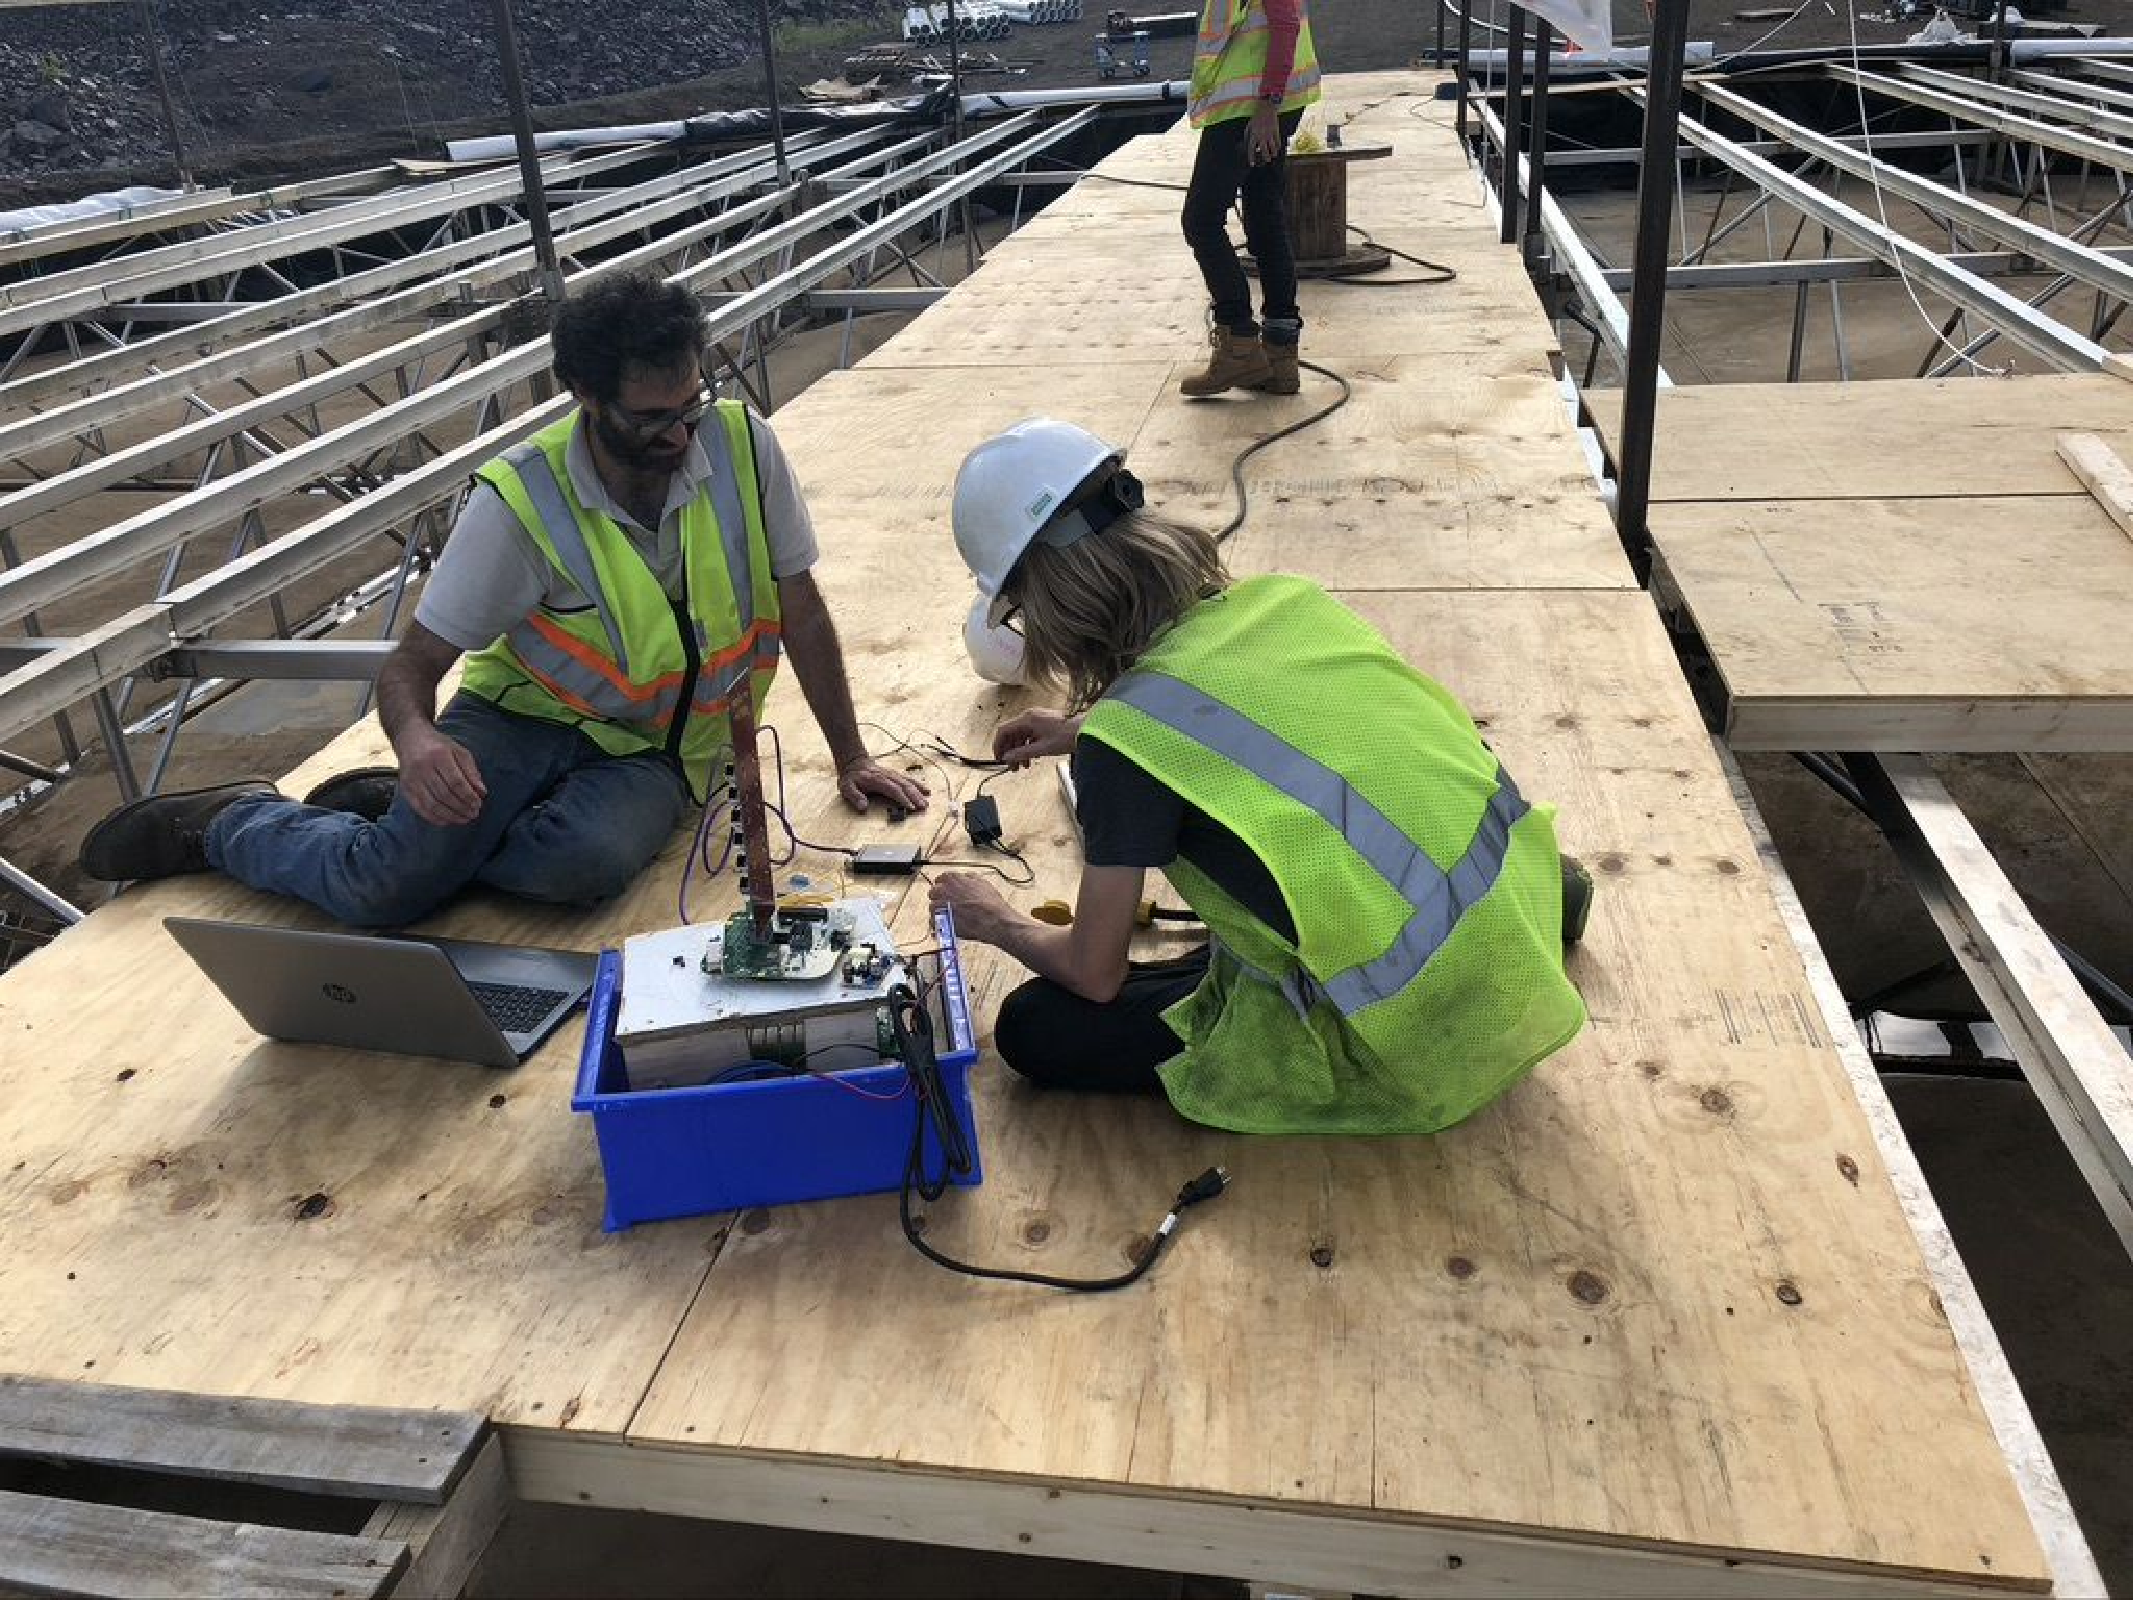
\includegraphics[height=5.6cm]{diagrams/4-chips/work1.pdf}%
    }
    \quad
    \subcaptionbox{\textsc{Pom} installation.}{%
        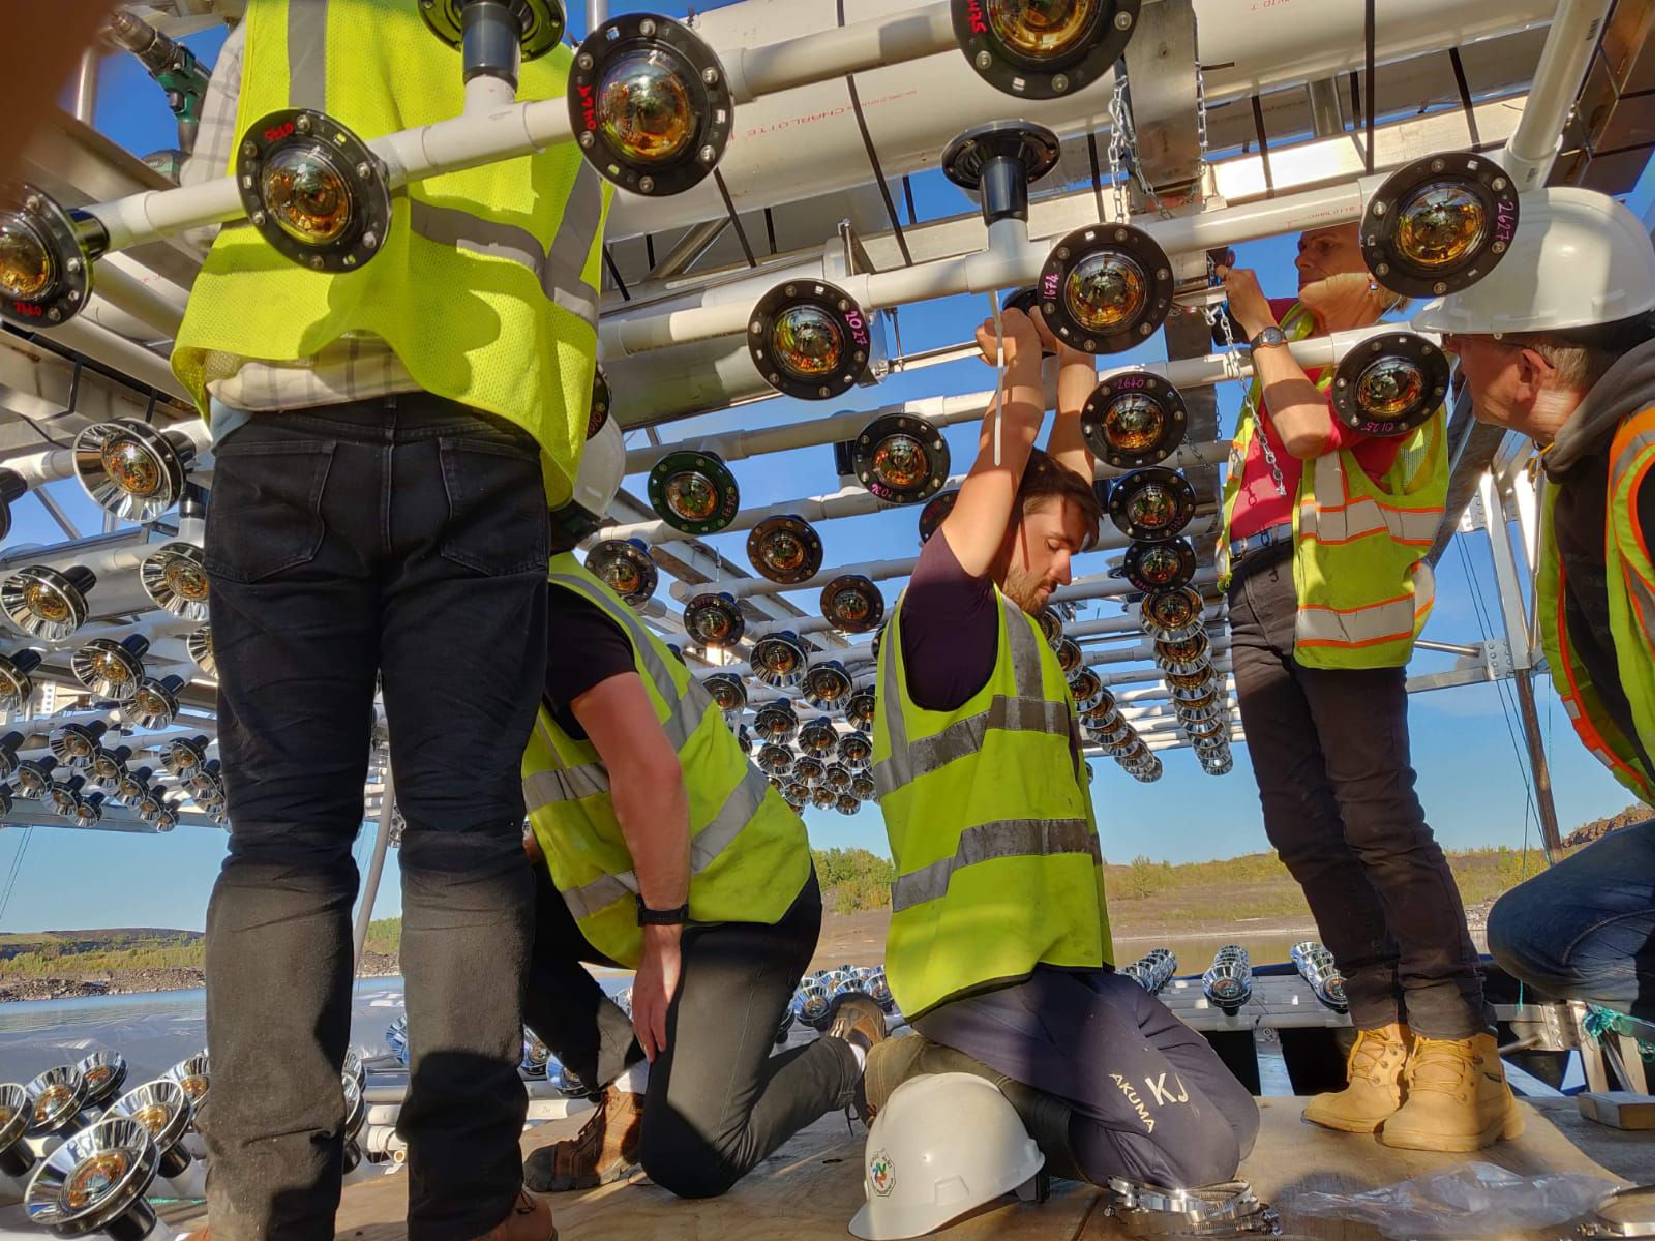
\includegraphics[height=5.6cm]{diagrams/4-chips/work4.pdf}%
    }
    \caption[More \chipsfive construction work]
    {More \chipsfive construction work.}
    \label{fig:work2}
\end{figure}

By late summer 2019, it became apparent that deployment of a fully instrumented \chipsfive would
be impossible before the pit started to freeze over in October. Therefore, the decision was taken
to only partially instrument the endcaps, leave the barrel walls bare, not include the veto
separation liner, and reduce the module height to \unit{8}{\text{m}}. In October 2019 this version
of \chipsfive, shown in Fig.~\ref{fig:complete}, was deployed into the Wentworth 2W pit.

Analysis of preliminary data was successful in isolating individual cosmic muon events, one of
which is shown in Fig.~\ref{fig:cosmic_event}. However, extensive data taking was paused due to a
deployment induced tear in the liner preventing filtration of the internal water. Given the
outbreak of the worldwide SARS-CoV-2 epidemic, all plans for work over the summer of 2020 were
suspended, including the essential repairs and instrumentation of the barrel walls. Plans for
summer 2021 are currently under review.

\begin{figure} % COMPLETE PICTURE DIAGRAM %
    \includegraphics[width=0.9\textwidth]{diagrams/4-chips/complete.pdf}
    \caption[Inside picture of \chipsfive just before deployment]
    {Inside picture of \chipsfive just before deployment, with a section of the total
        instrumentation shown. In total 56 Nikhef and 6 Madison \textsc{Pom}s were installed.
        Instead of being mounted on the upstream detector walls the Madison \textsc{Pom}s were
        mounted on the bottom-cap and can be seen in the foreground of the image. The flexible PVC
        tube pigtails and manifolds can also be seen connecting each \textsc{Pom} to the higher
        level DAQ electronics and power supply.}
    \label{fig:complete}
\end{figure}

\begin{figure} % COSMIC EVENT DIAGRAM %
    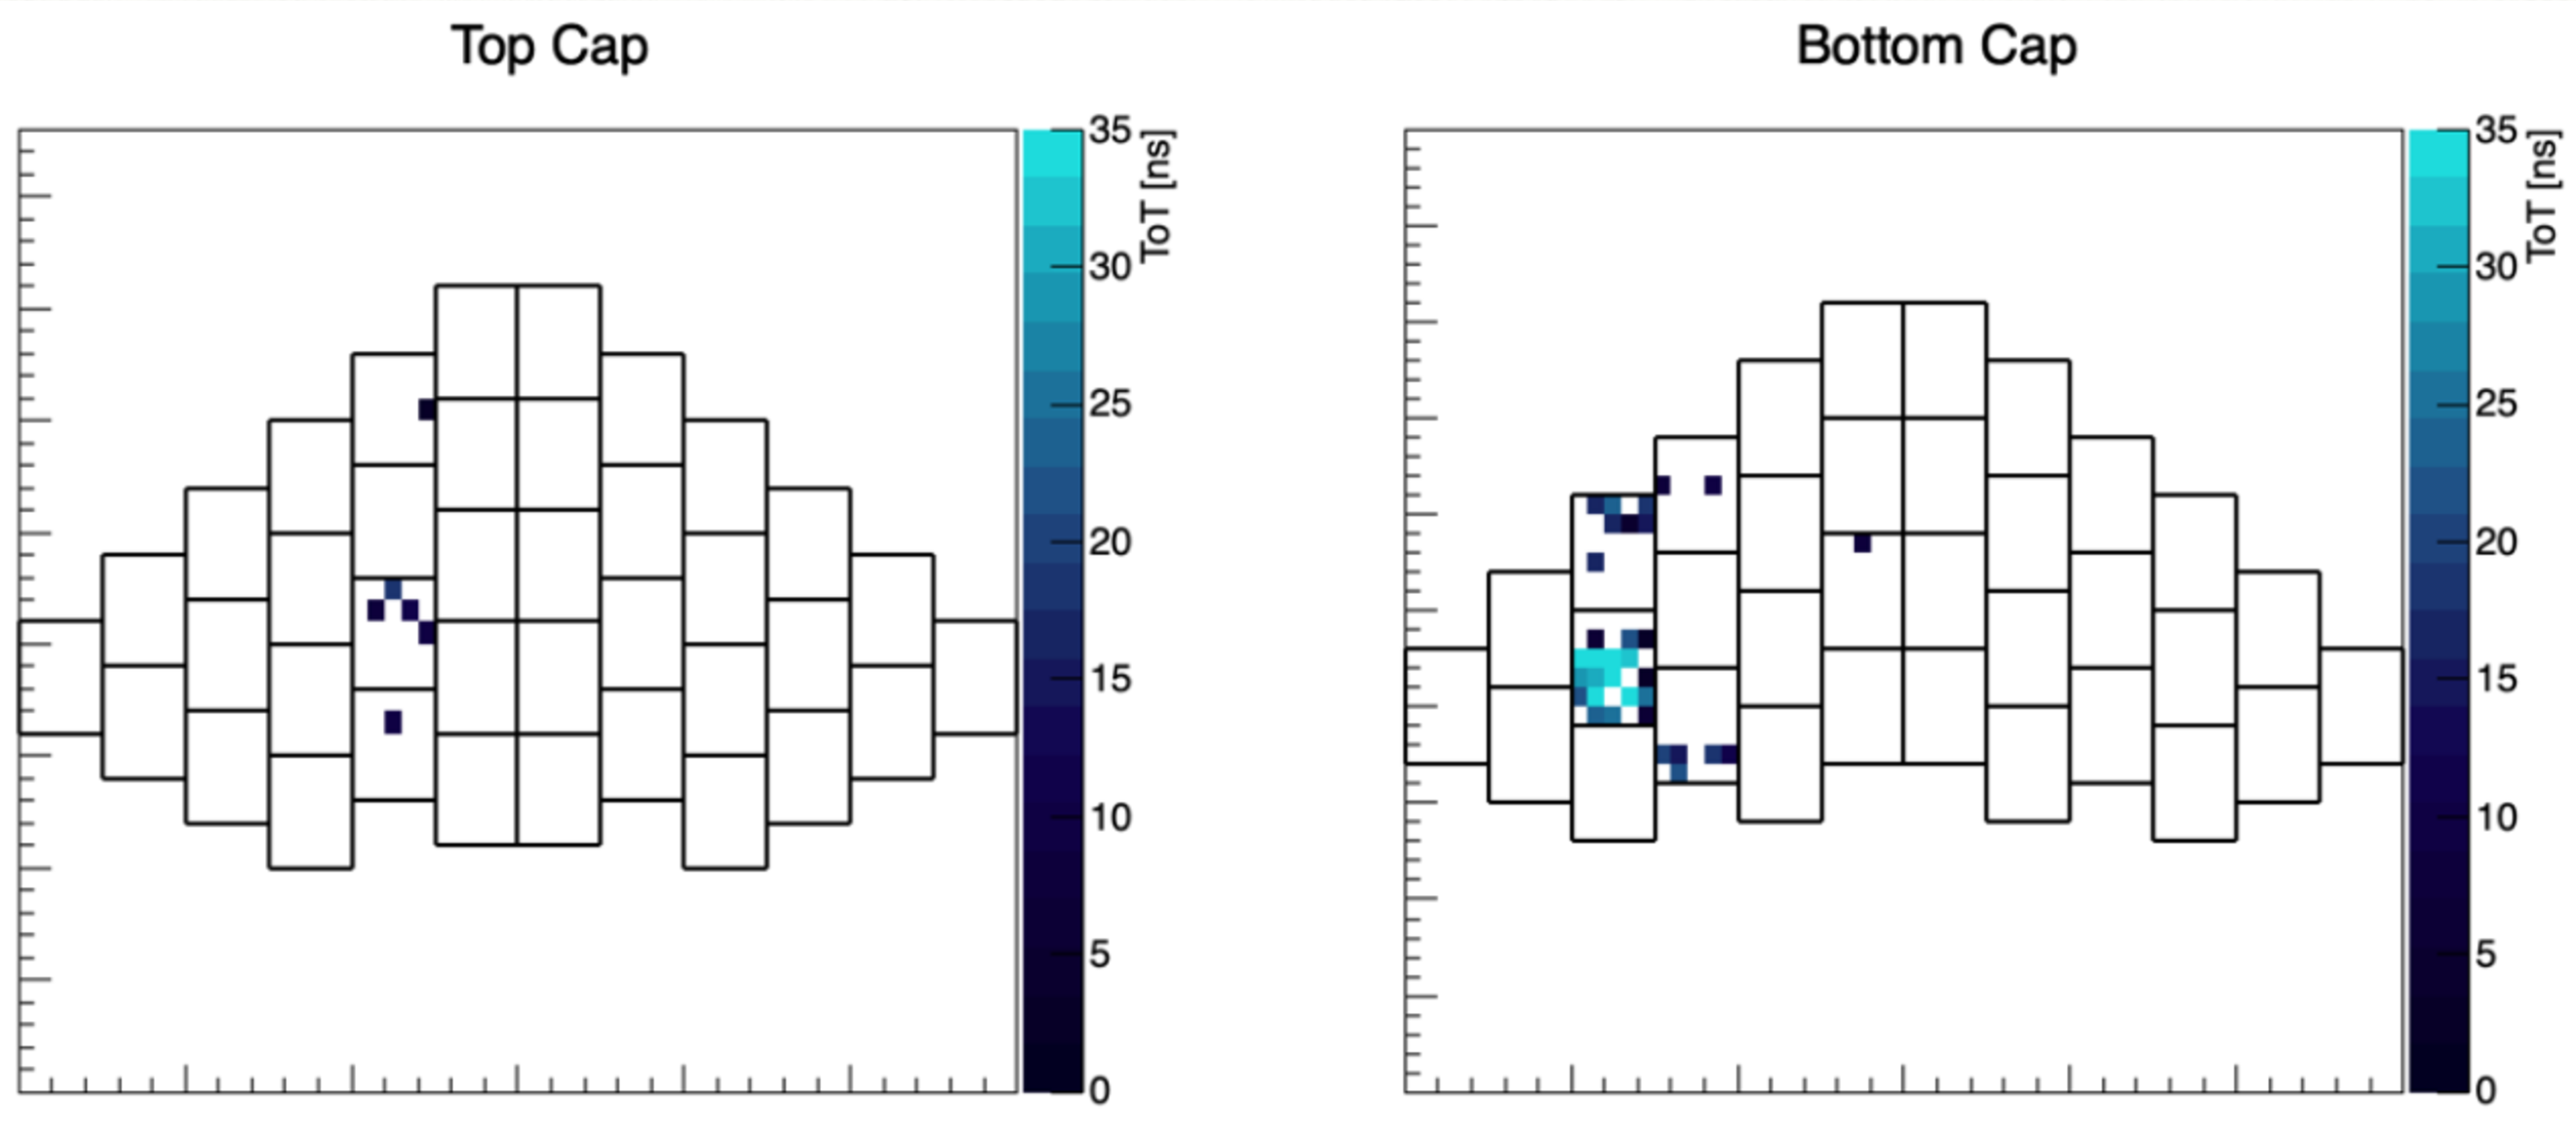
\includegraphics[width=\textwidth]{diagrams/4-chips/cosmic_event.pdf}
    \caption[A cosmic muon event recorded within \chipsfive]
    {A cosmic muon event recorded within \chipsfive, found by clustering hits in time. PMT hits
    from both the top-cap (left) and bottom-cap (right) are shown with the colour indicating the
    measured ToT value. Due to the small attenuation length of unfiltered water, only a single
    bottom-cap \textsc{Pom} has significant activity.}
    \label{fig:cosmic_event}
\end{figure}

\section{Detector simulation and event generation} %%%%%%%%%%%%%%%%%%%%%%%%%%%%%%%%%%%%%%%%%%%%%%%
\label{sec:chips_monte_carlo} %%%%%%%%%%%%%%%%%%%%%%%%%%%%%%%%%%%%%%%%%%%%%%%%%%%%%%%%%%%%%%%%%%%%

To describe the \chipsfive module and other \chips concept detectors in a simulated environment, a
Monte Carlo simulation framework is used. Monte Carlo detector simulation and event generation
methods are an indispensable tool within high energy particle physics. This is particularly true
during the design and prototyping phase of an experimental project when no real-world data is
available, as is predominantly the case with \chips. By matching the observables of a real-world
detector as close as possible, these methods allow for the optimisation of designs, the testing of
reconstruction techniques, and the study of physics sensitivities.

Here, a description of the detector simulation and the beam and cosmic event generation procedures
used by \chips are described. All are employed extensively for the work presented in
Chapter.~\ref{chap:cnn} and Chapter.~\ref{chap:results} of this thesis.

\subsection{Detector simulation} %%%%%%%%%%%%%%%%%%%%%%%%%%%%%%%%%%%%%%%%%%%%%%%%%%%%%%%%%%%%%%%%%
\label{sec:chips_monte_carlo_sim} %%%%%%%%%%%%%%%%%%%%%%%%%%%%%%%%%%%%%%%%%%%%%%%%%%%%%%%%%%%%%%%%

The detector simulation uses the WCSim water Cherenkov simulation package~\cite{wcsim2020} built
on top of the Geant4 simulation framework~\cite{agostinelli2003, allison2006, allison2016}.
Developed initially to simulate possible water Cherenkov detectors in the LBNF beam, WCSim is now
used more widely in the field. Heavily modified for the \chips project, WCSim allows for generic
water Cherenkov detector geometries to be easily loaded at runtime via a series of simple XML
configuration files. These changes allow for a broad range of detector geometries to be quickly
considered without recompilation of the code.

The simulation builds an n-sided, regular polygonal prism consisting of two endcaps and a barrel,
filled with water and lined with a low reflectivity \emph{blacksheet}. The geometry is separated
into \emph{regions} within both the barrel and endcaps, defined either by a list of barrel sides
or an opening angle respectively. Each region is filled with a unique base unit of geometry known
as the \emph{unit cell}, as shown in Fig.~\ref{fig:sim_geom}.

The unit cell defines a pattern of any number of PMTs, including their relative positions and in
which direction they face. The final geometry is built by tiling the defined regions with their
respective unit cell scaled to match the required regional photocathode coverage. Note that
although exact PMT positions are not used in this procedure, a given configuration will always
generate the same geometry (it is deterministic). In this work, the \chipsfive geometry is
generated with 28 sides and regions matching the boundary angles and photocathode coverage
detailed in Section.~\ref{sec:chips_detector_instrumentation}.

\begin{figure} % SIMULATION GEOM DIAGRAM %
    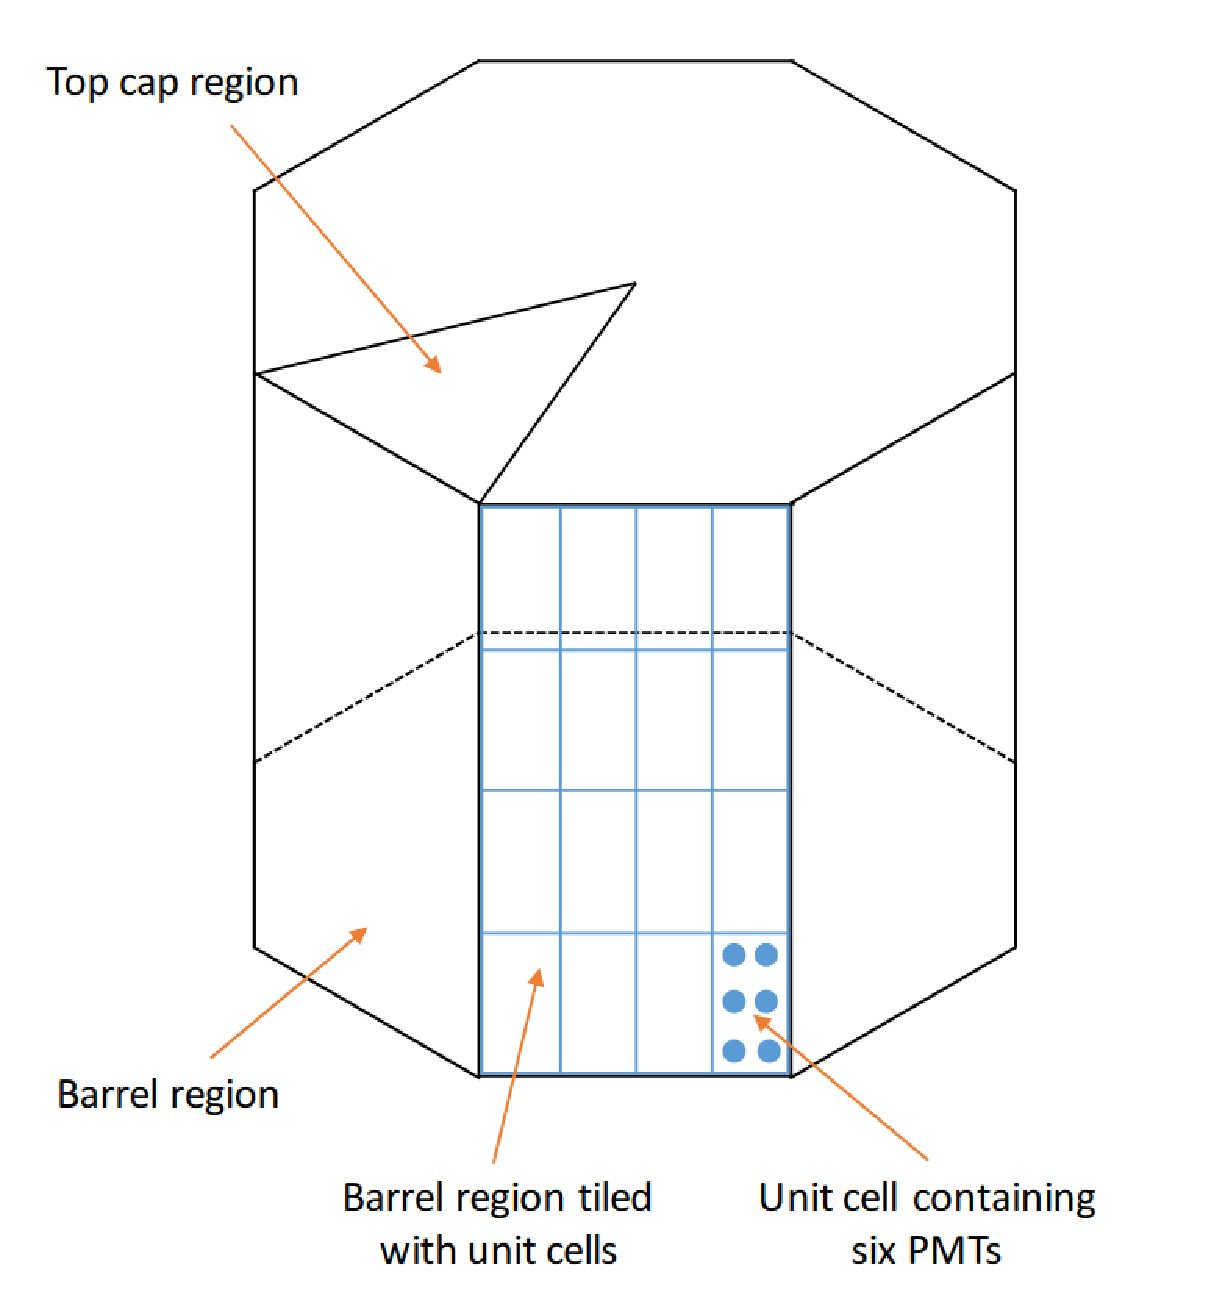
\includegraphics[width=0.5\textwidth]{diagrams/4-chips/sim_geom.pdf}
    \caption[Illustrative diagram of a WCSim detector geometry]
    {Illustrative diagram of a WCSim detector geometry. The endcap and barrel regions, tiled unit
        cells, and PMTs within a unit cell are all shown. Figure taken from
        Ref.~\cite{blake2016}.}
    \label{fig:sim_geom}
\end{figure}

The geometry shape, regions, and unit cells are defined in a configuration file. Additionally, a
file for PMT definitions containing their shape, time resolution, and quantum efficiency is also
used. Light-cones are described by a list of radial profile points in a further file. Although the
underlying Geant4 material properties are mostly hardcoded (taken from the Super-Kamiokande
simulation), values within yet another configuration file are used to scale them. This scaling
controls the water absorption, scattering (Rayleigh and Mie) lengths, and both the blacksheet and
PMT glass reflectivity. In this work a photon attenuation length of \unit{50}{\text{m}} at
\unit{405}{\text{nm}} is used with negligible scattering, the blacksheet reflectivity is set to be
4\% and the PMT glass reflectivity 24\%.

A veto volume can also be defined. The veto is built as either a concentric shell around the whole
inner volume with a given thickness, or solely above the top-cap with a given height. Any PMTs
defined as facing outwards within a unit cell look into the veto volume instead of the inner
volume. In this work, the \chipsfive geometry is given a top-cap veto of height
\unit{1.3}{\text{m}} with a photocathode coverage matching that described in
Section.~\ref{sec:chips_detector_instrumentation}.

Once the full generation of the Geant4 geometry is complete, the final state tracks for each
successive event to be simulated are loaded from either the beam or cosmic event generator files
described next in Section.~\ref{sec:chips_monte_carlo_beam} and
Section.~\ref{sec:chips_monte_carlo_cosmic}. Beam event vertices are randomly placed within the
inner detector volume, while cosmic vertices are set at \unit{1}{\text{m}} above the detector
volume. WCSim then simulates the passage of all particles through the detector materials, with
interactions, decays, and Cherenkov emission all taken into account.

Whenever a photon is calculated to have hit the photocathode of a PMT, an angular dependent
acceptance efficiency is applied to see if it is recorded. If accepted, all hits within
\unit{200}{\text{ns}} windows are grouped to form a single recorded hit, with a smeared first hit
time used as the recorded time. The standard WCSim methodology is used to determine the total
output charge of the hit given the number of incident photons. This procedure involves a single
photoelectron charge distribution being repeatedly probed for each photon, before the combined sum
is returned~\cite{tutorial2020}.

By sampling this procedure multiple times, the output charge probability distribution given the
number of incident photons can be generated, as shown in Fig.~\ref{fig:digitisation}. The reverse
likelihood function of an actual number of incident photons given a measured digitised charge is
also shown (with a lower value being more likely). The reverse likelihood function is used for the
standard reconstruction methods outlined in Section.~\ref{sec:cnn_old_reco}.

\begin{figure} % DIGI DIAGRAM %
    \centering
    \subcaptionbox{\label{fig:digi_method}}{%
        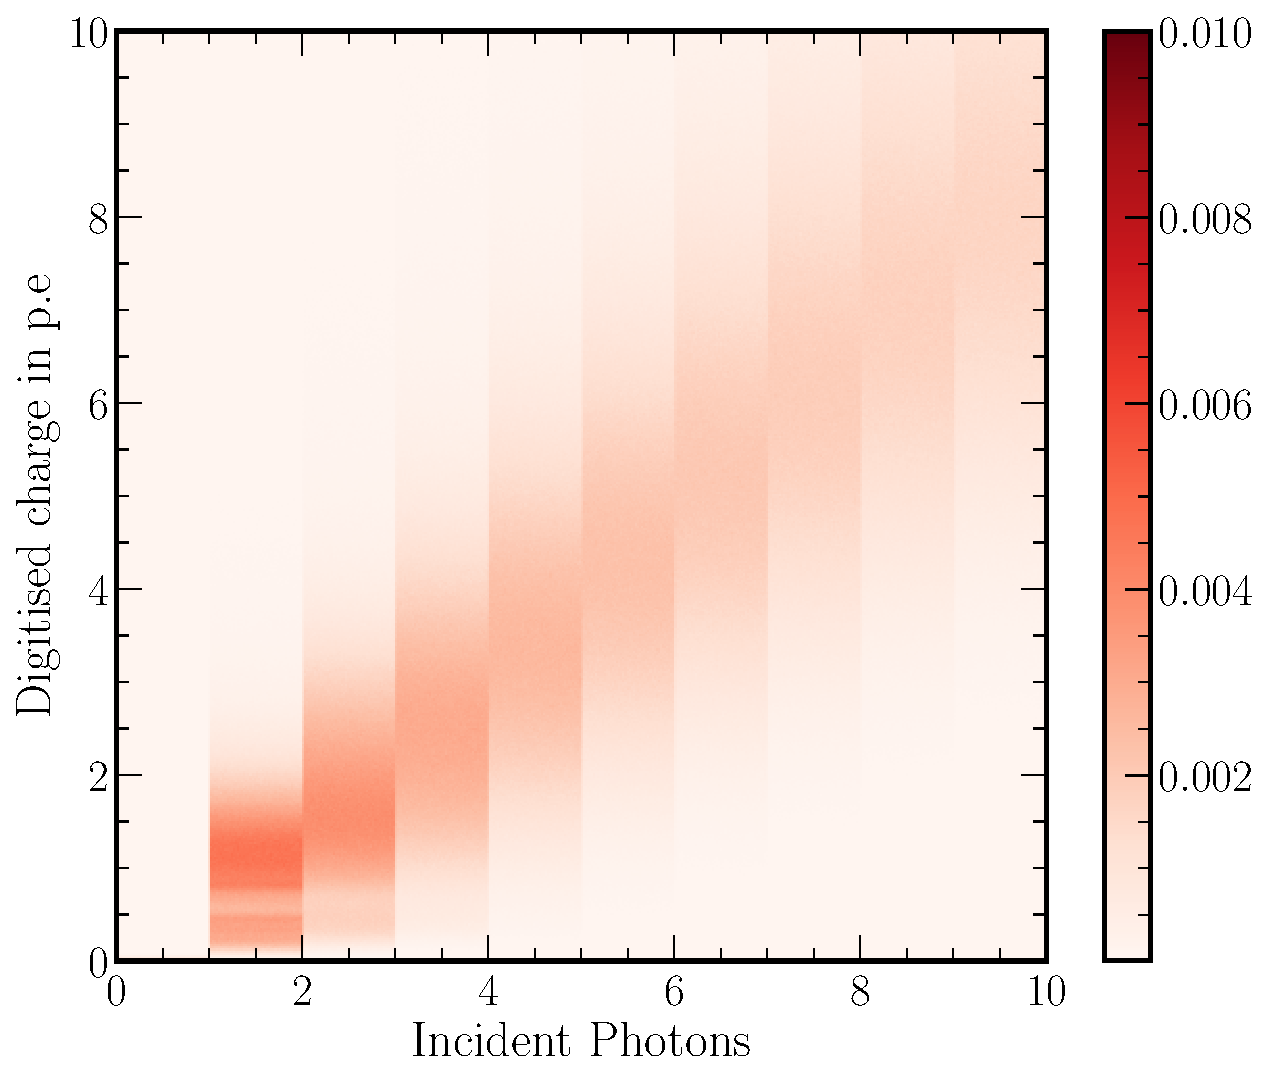
\includegraphics[height=6cm]{diagrams/4-chips/digi_method.pdf}%
    }
    \quad
    \subcaptionbox{\label{fig:digi_likelihood}}{%
        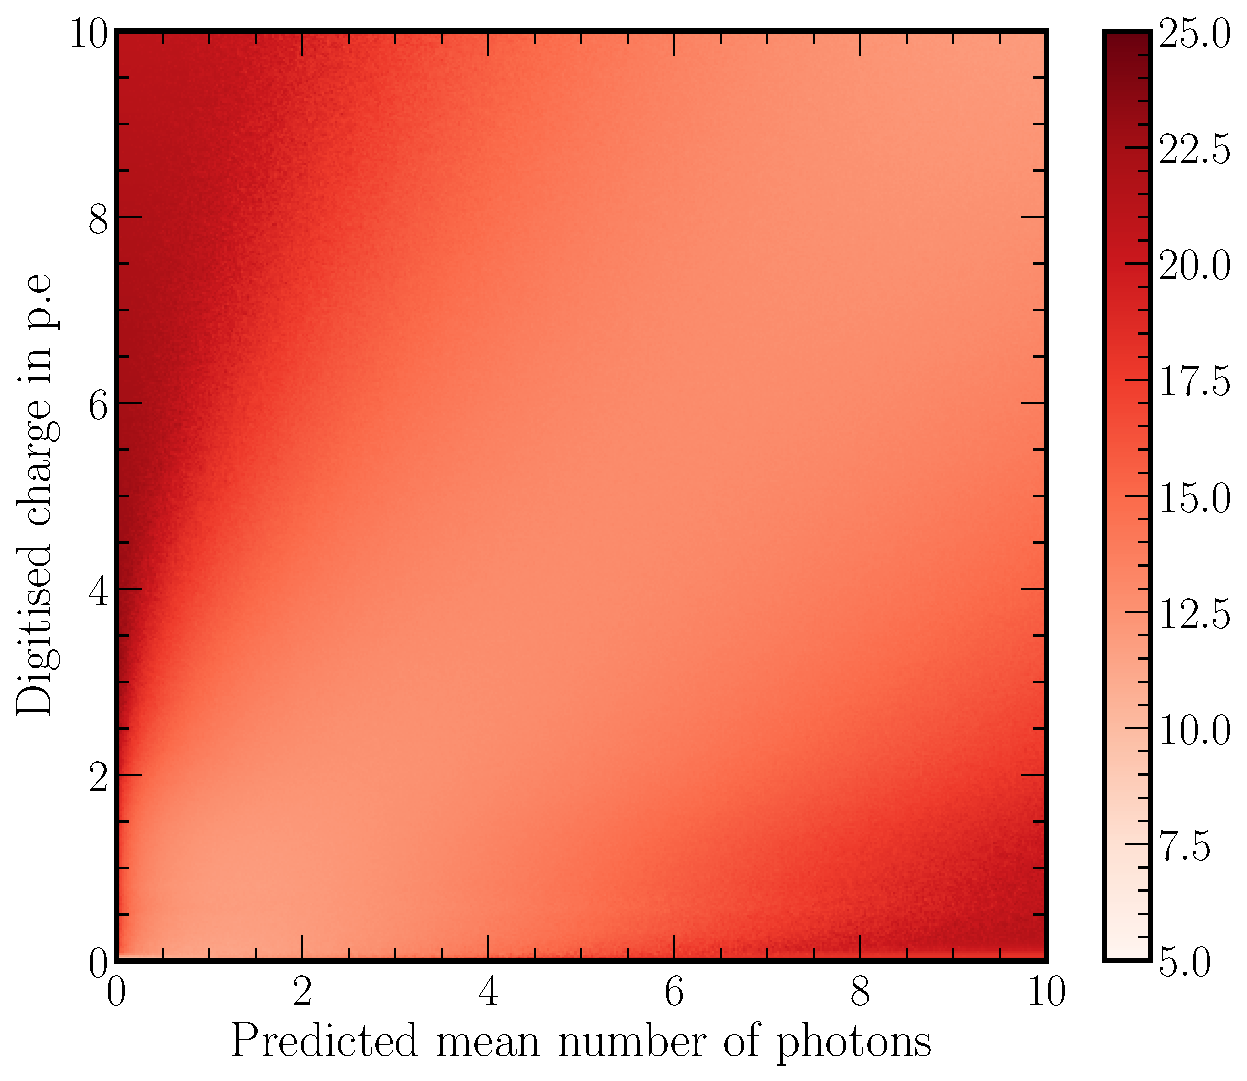
\includegraphics[height=6cm]{diagrams/4-chips/digi_likelihood.pdf}%
    }
    \caption[Detector simulation PMT digitisation function]
    {The probability of a digitised output charge given an incident number of photons used within
    the detector simulation is shown in (a). The reverse function, showing the likelihood of a
    measured digitised charge being caused by a number of incident photons is shown in (b).}
    \label{fig:digitisation}
\end{figure}

The simulated PMT hits for each event are stored in an output file along with truth information
and track descriptions. A full event takes approximately three seconds to simulate on a standard
batch farm computing node.

\subsection{Beam event generation} %%%%%%%%%%%%%%%%%%%%%%%%%%%%%%%%%%%%%%%%%%%%%%%%%%%%%%%%%%%%%%%
\label{sec:chips_monte_carlo_beam} %%%%%%%%%%%%%%%%%%%%%%%%%%%%%%%%%%%%%%%%%%%%%%%%%%%%%%%%%%%%%%%

The expected flux of beam neutrinos at the \chipsfive detector location, shown in
Fig.~\ref{fig:flux}, is generated using the existing beam simulation written for the \numi
experiments. Using the generated fluxes as input, the \textsc{Genie} neutrino event generator
(version 3.0.6)~\cite{andreopoulos2009, andreopoulos2015} is used to generate beam neutrino
events. Default neutrino cross-sections on water provided by \textsc{Genie} are used during
generation. All initial, intermediate, and final state particle tracks for each event are stored
as output in a NUANCE formatted file for use in the detector simulation. Note that unoscillated
input fluxes are used such that analyses samples must be later weighted to match the desired
oscillated neutrino composition.

\begin{figure} % CHIPS FLUX DIAGRAM %
    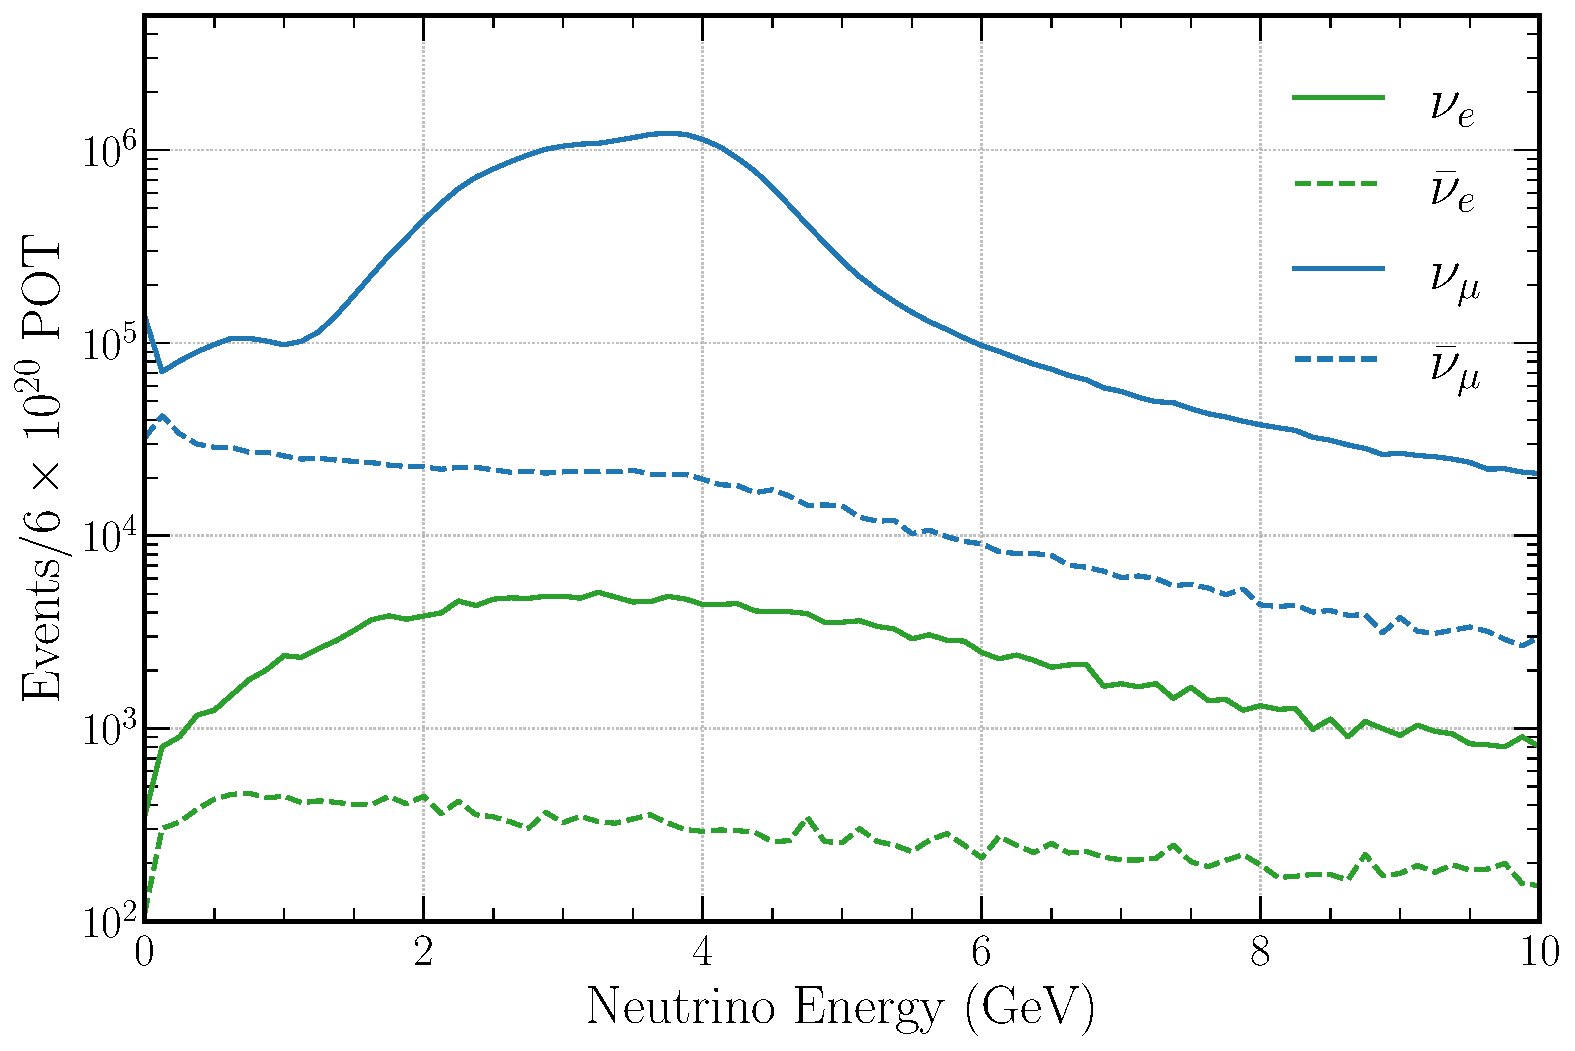
\includegraphics[width=0.7\textwidth]{diagrams/4-chips/flux.pdf}
    \caption[\numi neutrino flux at the \chipsfive detector location]
    {The neutrino mode (forward horn current) \numi beam neutrino energy spectrum at the
        \chipsfive detector module location. Shown are the individual contributions from the
        different neutrino types and signs. No cross-sections or oscillations have been applied.}
    \label{fig:flux}
\end{figure}

\subsection{Cosmic event generation} %%%%%%%%%%%%%%%%%%%%%%%%%%%%%%%%%%%%%%%%%%%%%%%%%%%%%%%%%%%%%
\label{sec:chips_monte_carlo_cosmic} %%%%%%%%%%%%%%%%%%%%%%%%%%%%%%%%%%%%%%%%%%%%%%%%%%%%%%%%%%%%%

The Cosmic-Ray Shower Library (CRY)~\cite{hagmann2012_1, hagmann2012_2} is used for cosmic ray
event generation. Both the solar cycle and Earth's geomagnetic field are taken into account, with
the \mbox{\chipsfive} latitude ($47.56^{\circ}$ N) and deployment date (30th October 2019) used as
input. Single muons are generated at sea level by CRY within a \unit{1}{\text{km}} by
\unit{1}{\text{km}} area, with the detector at it's centre. Note that only single muon events (the
dominant cosmic component) are considered for simplicity.

Assuming a \chipsfive overburden of \unit{50}{\text{m}} and a \unit{2.2}{\MeV/\text{cm}^{2}} muon
energy loss in water as suggested by Ref.~\cite{klimushin2001} the muon parameters are updated to
estimate their values at \unit{1}{\text{m}} above the detector. All muons whose path does not
cross the detector volume or do not have sufficient energy to reach the detector are
discarded~\cite{chipsgen2020}. All accepted muon tracks are stored as output in a NUANCE formatted
file for use in the detector simulation.

To use generated cosmic events in analysis, studies have looked at the likely cosmic rate for
\chips detector modules at different water overburden depths~\cite{son2013}. In this work, the
fits shown in Fig.~\ref{fig:cosmic_rate} for a cylindrical detector of both height and diameter
\unit{24}{\text{m}} are used to estimate a \chipsfive cosmic muon rate of \unit{11.8}{\text{KHz}}
at \unit{50}{\text{m}} of overburden.

Given the \unit{10}{\micro\text{s}} long \numi beam spill occurring every
\unit{1.33}{\text{seconds}}, an in spill cosmic rate of $\sim2.1$ million events per year is
calculated with an in spill occupancy of 9\%. Considering a typical event takes
$\sim$\unit{100}{\text{ns}} to unfold, there is approximately a 0.3\% chance that any beam event
overlaps with a cosmic muon. This low coincidence shows just how powerful a short beam spill can
be at reducing the significant cosmic background.

\begin{figure} % COSMIC RATE DIAGRAM %
    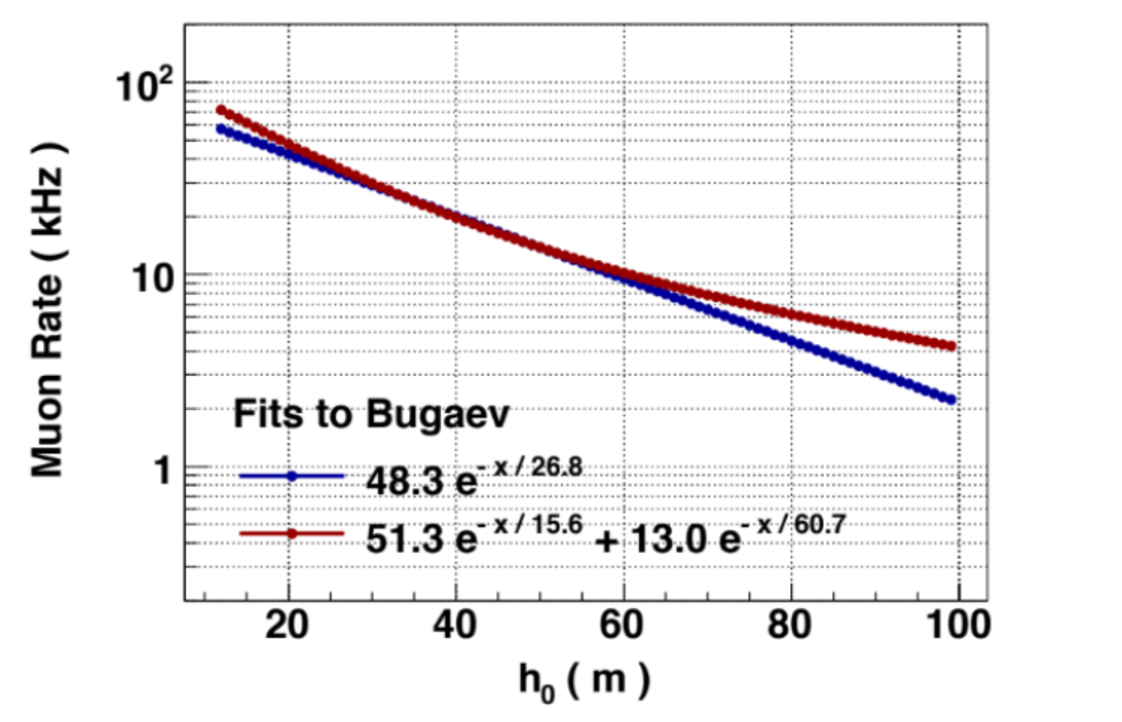
\includegraphics[width=0.6\textwidth]{diagrams/4-chips/cosmic_rate.pdf}
    \caption[Expected \chipsfive cosmic muon rate as a function of water overburden depth]
    {Expected cosmic muon rate as a function of water overburden depth for a \unit{24}{\text{m}}
        high and \unit{24}{\text{m}} wide \chips detector module. Shown are fits made to the work
        originally conducted in Ref.~\cite{bugaev1998}. Figure taken from Ref.~\cite{son2013}.}
    \label{fig:cosmic_rate}
\end{figure}